% SIAM Article Template
\documentclass[review,onefignum,onetabnum]{siamart190516}

% Information that is shared between the article and the supplement
% (title and author information, macros, packages, etc.) goes into
% ex_shared.tex. If there is no supplement, this file can be included
% directly.

% SIAM Shared Information Template
% This is information that is shared between the main document and any
% supplement. If no supplement is required, then this information can
% be included directly in the main document.


% Packages and macros go here
\usepackage{lipsum}
\usepackage{amsfonts}
\usepackage{graphicx}
\usepackage{epstopdf}
\usepackage{amsmath}
\usepackage{subcaption}
\usepackage{pgfplots}

%\usepackage{amsmath,amsthm}
%\usepackage[noend]{algorithmic}
%\usepackage{algorithmic}
\usepackage[algo2e, ruled, noend, linesnumbered]{algorithm2e}
%\usepackage[algo2e, ruled, vlined]{algorithm2e}
\usepackage{bm}
\ifpdf
  \DeclareGraphicsExtensions{.eps,.pdf,.png,.jpg}
\else
  \DeclareGraphicsExtensions{.eps}
\fi

\usepackage{placeins}
\usepackage{multirow}

% Add a serial/Oxford comma by default.
\newcommand{\creflastconjunction}{, and~}
\newcommand{\nor}[1]{\left\|#1\right\|}

% Used for creating new theorem and remark environments
\newsiamremark{remark}{Remark}
\newsiamremark{hypothesis}{Hypothesis}
\crefname{hypothesis}{Hypothesis}{Hypotheses}
\newsiamthm{claim}{Claim}
\newsiamthm{prop}{Proposition}
\newsiamthm{defn}{Definition}
\newsiamthm{thm}{Theorem}
\newsiamthm{cor}{Corollary}
\newsiamthm{lem}{Lemma}


\newcommand{\norm}[1]{\|#1\|}


% Sets running headers as well as PDF title and authors
\headers{Matrix-free PSF approximation}{N. Alger, T. Hartland, N. Petra, and O. Ghattas}

% Title. If the supplement option is on, then "Supplementary Material"
% is automatically inserted before the title.
\title{Matrix-free point spread function approximation of operators with locally supported non-negative integral kernels, with application to Hessians in PDE constrained inverse problems\thanks{Submitted to the editors DATE.
\funding{This research was supported by the National Science Foundation under Grant No. DMS-1840265 and CAREER-1654311.}}}

% Authors: full names plus addresses.
\author{Nick Alger\thanks{Oden Institute, The University of Texas at Austin, Austin, TX 
  (\email{nalger@oden.utexas.edu}).}
\and Tucker Hartland\thanks{Department of Applied Mathematics, University of California, Merced, Merced, CA. 
	(\email{thartland@ucmerced.edu}).}
\and Noemi Petra\thanks{Department of Applied Mathematics, University of California, Merced, Merced, CA. 
  (\email{npetra@ucmerced.edu}).}
\and Omar Ghattas\thanks{Oden Institute, The University of Texas at Austin, Austin, TX 
	(\email{omar@oden.utexas.edu}).}}

\newcommand{\Aop}{\mathcal{A}}
\newcommand{\AopPc}{\mathcal{A}_\text{pc}}
\newcommand{\AopPcMesh}{\mathcal{A}_\text{pc}^h}

\newcommand{\Aker}{\Phi}
\newcommand{\AkerPc}{\Phi_\text{pc}}
\newcommand{\AkerPcMesh}{\Phi_\text{pc}^h}

\newcommand{\AkerPcMat}{\mathbf{\Phi}_\text{pc}}

\newcommand{\Amat}{\mathbf{A}}
\newcommand{\AmatPc}{\mathbf{A}_\text{pc}}
\newcommand{\AmatPcSym}{\mathbf{A}_\text{pc}^\text{sym}}
\newcommand{\AmatPcSymPlus}{\mathbf{A}_\text{pc}^{\text{sym}+}}

\newcommand{\diraccomb}{\xi}
\newcommand{\combresponse}{\eta}
\newcommand{\weakadmconst}{C}
\newcommand{\horizinterpolant}{\theta}
\newcommand{\interpolatedvalues}{b}
\newcommand{\firstgreens}{G}
\newcommand{\secondgreens}{F}
\newcommand{\impulseresponse}{\phi}
\newcommand{\convkernel}{\varphi}
\newcommand{\febasis}{\psi}
\newcommand{\ratfct}{R}
\newcommand{\ratpole}{\omega}
\newcommand{\ratcoeff}{c}
\newcommand{\massmatrix}{\mathbf{M}}
\newcommand{\spatialvol}{V}
\newcommand{\spatialmean}{\mu}
\newcommand{\spatialcov}{\Sigma}
\newcommand{\genericdistribution}{\rho}
\newcommand{\pointbatch}{S}
\newcommand{\pointinteractionmatrix}{S}
\newcommand{\gdim}{d}
\newcommand{\fedim}{N}
\newcommand{\convrank}{r}
\newcommand{\hrank}{k_h}
\newcommand{\nbatch}{n_b}
\newcommand{\numnbr}{k_{n}}
\newcommand{\ratord}{l}
\newcommand{\nsamplepts}{m}
\newcommand{\ptsonebatch}{s}
\newcommand{\classicalrank}{r}
\newcommand{\secondgreenscoeff}{\beta}
\newcommand{\constcoeff}{\alpha}
\newcommand{\colcluster}{\mathtt{c}}
\newcommand{\rowcluster}{\mathtt{r}}
\newcommand{\icedomain}{U}
\newcommand{\basalfriction}{{q}}
\newcommand{\normalvec}{\nu}
\newcommand{\searchdir}{{\widehat{\basalfriction}}}
\newcommand{\preconditioner}{\widetilde{H}}
\newcommand{\candidatepts}{X}
\newcommand{\eigenvectormatrix}{P}
\newcommand{\candidatepoint}{x}
\newcommand{\velocity}{v}
\newcommand{\pressure}{p}
\newcommand{\rbfweight}{c}
\newcommand{\stress}{\sigma}
\newcommand{\tangentop}{T}
\newcommand{\strain}{\varepsilon}
\newcommand{\bodyforce}{f}
\newcommand{\observations}{y}
\newcommand{\rbf}{\varphi}
\newcommand{\fepoint}{\zeta}
\newcommand{\stokesrobincoeff}{{s}}
\newcommand{\regrobincoeff}{{s}}
\newcommand{\regrhs}{{f}}

\newcommand*{\vertbar}{\rule[-1ex]{0.5pt}{2.5ex}}
\newcommand*{\horzbar}{\rule[.5ex]{2.5ex}{0.5pt}}

\usepackage{amsopn}
\DeclareMathOperator{\diag}{diag}
\DeclareMathOperator{\interpolate}{Interpolate}
\DeclareMathOperator{\Span}{span}
\DeclareMathOperator{\Var}{Var}
\DeclareMathOperator{\vol}{vol}
\DeclareMathOperator{\avg}{avg}
\DeclareMathOperator*{\argmax}{arg\,max}
\DeclareMathOperator*{\argmin}{arg\,min}
\DeclareMathOperator{\dist}{dist}
\DeclareMathOperator{\diam}{diam}
\DeclareMathOperator{\nbrs}{nbrs}

\newcommand{\computediracresponse}[1]{\text{compute\_dirac\_comb\_response}\left( #1 \right)}
\newcommand{\ellipsoidsintersect}[2]{\text{ellipsoids\_intersect}\left( #1, #2 \right)}
\newcommand{\choosebatch}[1]{\text{choose\_sample\_point\_batch}\left( #1 \right)}
\newcommand{\computekernelentries}[2]{\text{compute\_approximate\_kernel\_entries}\left( #1 , #2 \right)}
\newcommand{\computeweightingentries}[1]{\text{compute\_weighting\_function\_entries}\left( #1 \right)}

\DeclareFontFamily{U}{wncy}{}
\DeclareFontShape{U}{wncy}{m}{n}{<->wncyr10}{}
\DeclareSymbolFont{mcy}{U}{wncy}{m}{n}
\DeclareMathSymbol{\Sh}{\mathord}{mcy}{"58} 

\SetEndCharOfAlgoLine{}
%\SetKwIF{If}{ElseIf}{Else}{if}{}{else if}{else}{end if}

%\renewcommand{\algorithmicrequire}{\textbf{Input:}}
%\renewcommand{\algorithmicensure}{\textbf{Output:}}


%%% Local Variables: 
%%% mode:latex
%%% TeX-master: "ex_article"
%%% End: 


% Optional PDF information
\ifpdf
\hypersetup{
  pdftitle={Fast matrix-free approximation of locally translation invariant operators that have locally supported non-negative integral kernels, with application to Hessians in PDE-constrained inverse problems},
  pdfauthor={N. Alger, N. Petra, T. Hartland, and O. Ghattas}
}
\fi

% The next statement enables references to information in the
% supplement. See the xr-hyperref package for details.

\externaldocument{localpsf_supplement}

% FundRef data to be entered by SIAM
%<funding-group specific-use="FundRef">
%<award-group>
%<funding-source>
%<named-content content-type="funder-name"> 
%</named-content> 
%<named-content content-type="funder-identifier"> 
%</named-content>
%</funding-source>
%<award-id> </award-id>
%</award-group>
%</funding-group>

\begin{document}

\maketitle

% REQUIRED
\begin{abstract}
	We present a fast matrix-free method for computing hierarchical matrix (H-matrix) approximations of operators that have locally supported non-negative integral kernels. Such operators arise, for example, as Schur complements in Schur complement methods for solving partial differential equations (PDEs), Poincare-Steklov operators in domain decomposition methods, covariance operators in spatial statistics, blurring operators in imaging, and Hessians in distributed parameter PDE-constrained inverse problems. 
%	H-matrix approximations are highly desirable because 
	Fast H-matrix methods can add, multiply, invert, and factorize H-matrices, compute matrix-vector products, solve linear systems, and perform other useful matrix computations. 
%	The computational cost of these operations is $O(N \log^a N)$, where the matrix is $N\times N$, and $a \in \{1,2,3\}$. 
%	Classical H-matrix construction methods 
%	require evaluating the integral kernel $O(N \log N)$ times, but this is not feasible 
%	are infeasible for large-scale problems in which the operator is only accessible via matrix-vector products (``matrix-free''), because these methods require evaluating the integral kernel of the operator at a large number of points. We overcome this problem by c
	Our method computes impulse responses of the operator at a collection of scattered points, then interpolates these known impulse responses to evaluate entries of the integral kernel at other points where the impulse response is not known. 
%	We improve upon classical product-convolution approximations by translating with respect the estimated mean of the impulse response, rather than the location of the impulse response point source. 
	Impulse responses are computed by applying the operator to a small number of Dirac combs associated with ``batches'' of point sources. 
%	We construct a-priori ellipsoid estimates of the supports of the impulse responses (i.e., support ellipsoids are estimated \emph{before} any impulse responses have been computed). 
	By solving an ellipsoid packing problem, we choose as many points as possible per batch, while ensuring that the supports of the impulse responses within each batch do not overlap. 
	We apply the method to approximate Hessians in large-scale PDE-constrained inverse problems with highly informative data. Numerical results demonstrate that our method substantially outperforms existing state-of-the-art Hessian approximation methods which are based on low-rank approximation. We are able to form high quality approximations of high rank operators using only a small number of operator actions products.
\end{abstract}

% REQUIRED
\begin{keywords}
  
\end{keywords}

% REQUIRED
\begin{AMS}
  
\end{AMS}

\section{Introduction}
\label{sec:intro}

We present a fast matrix free method for approximating operators that have locally supported non-negative integral kernels. Such operators arise as Schur complements in Schur complements methods for solving partial differential equations (PDEs) \cite{TOBYPAPER}, Poincare-Steklov operators in domain decomposition methods (e.g., Dirichlet-to-Neumann maps), covariance operators in spatial statistics, blurring operators in imaging, and Hessians in distributed parameter PDE-constrained optimization and inverse problems.

Let $\Omega \subset \mathbb{R}^d$ be a bounded domain (in applications typically $\gdim=1$, $2$, or $3$) and let $\Aop:L^2(\Omega)\rightarrow L^2(\Omega)'$ be an integral operator of the following form:
\begin{equation}
	\label{eq:kernel_representation}
	(\Aop u)(v) := \int_\Omega \int_\Omega v(y) \Aker(y,x) u(x) dx dy.
\end{equation}
The function $\Aker:\Omega \times \Omega \rightarrow \mathbb{R}$ is the integral kernel, $\Aop u \in L^2(\Omega)'$ is the linear functional that results from applying $\Aop$ to $u\in L^2(\Omega)$, and $\left(\Aop u\right)(v)$ is the scalar that results from applying that linear functional to $v \in L^2(\Omega)$. We seek to approximate operators $\Aop$ that are accessible \emph{matrix-free}. That is,
%access to $\Aop$ is available through ``operator actions.'' That is,
we have a black-box computational procedure through which we may evaluate the maps
\begin{equation*}
u \mapsto\Aop u \qquad \text{and} \qquad v \mapsto \Aop^Tv
\end{equation*} 
for arbitrary functions $u$ and $v$, but we cannot easily compute kernel entries $\Aker(y,x)$. In applications, evaluating these maps may involve iteratively solving a large linear system, timestepping, or performing some other nontrivial computational procedure. After discretization, $\Aop$ becomes a dense matrix that is typically too large to be built and stored. This property is called ``matrix-free'' because at the discrete level it means one can compute matrix-vector products with the matrix representation of $\Aop$, but cannot easily compute individual matrix entries.
%After discretization (see Appendix \ref{app:discretized_operations}), $\Aop$ becomes a dense matrix, $\bm{A}$, that is typically too large to be built and stored. This property is called ``matrix-free'' because at the discrete level it means that one can perform matrix-vector products of $\bm{A}$ and $\bm{A}^T$ with arbitrary vectors, but one cannot easily\footnote{One could compute $\bm{v} = \bm{A}\bm{e}_j$, where $\bm{e}_j=(0,\dots,0,1,0,\dots,0)$ is the unit vector which has $j^\text{th}$ component equal to one and all other components equal to zero, then extract $\bm{A}_{ij} = \bm{v}_i$. However, this process is wasteful because one computes the entire vector $\bm{v}$, then discards all but one component.} access matrix entries $\bm{A}_{ij}$. 

%For example, in reduced space approaches to PDE-constrained optimization and inverse problems, Hessian information is available only through the application of the Hessian to vectors, and one such Hessian application requires solving two PDEs \cite{HESSIANADJOINT}. 

Our method, described in Section \ref{sec:method}, belongs to a class of methods that approximate an operator by interpolating impulse responses of the operator associated with a scattered collection of points. The \emph{impulse response} of $\Aop$ associated with the point $x$ is the function $\impulseresponse_x:\Omega \rightarrow \mathbb{R}$, 
\begin{equation}
\label{eq:impulse_response_defn}
\impulseresponse_x(y) := \Aker(y, x),
\end{equation} 
which results from keeping $x$ fixed and viewing $\Phi(y,x)$ as a function of $y$.
%for a collection of points $x_i$ scattered throughout $\Omega$.
%Further, let $\impulseresponse_x:\Omega \rightarrow \mathbb{R}$,
%\begin{equation}
%\label{eq:impulse_response_defn}
%\impulseresponse_x(y) := \Aker(y, x),
%\end{equation} 
%be the \emph{impulse response} of $\Aop$ at $x$. 
The function $\impulseresponse_x$ is called the impulse response because straightforward analysis shows that it may be expressed as follows:
\begin{equation}
\label{eq:impulse_response_delta_action}
\impulseresponse_x = \left( \Aop \delta_x^* \right)^*,
\end{equation}
where $\delta_x$ is the the delta distribution (i.e., point source, impulse) centered at $x$, $\Aop \delta_x^* \in L^2(\Omega)'$ is an abuse of notation that denotes the result of applying $\Aop$ to the distribution $\delta_x$, and $\left( \Aop \delta_x^* \right)^* \in L^2(\Omega)$ denotes the Riesz representation of $\Aop \delta_x^*$ with respect to the $L^2$ inner product.\footnote{Recall that the Riesz representative of a functional $\sigma \in L^2(\Omega)'$ with respect to the $L^2$ inner product is the unique function $\sigma^* \in L^2(\Omega)$ such that $\sigma(v) = \left(\sigma^*,v\right)_{L^2(\Omega)}$ for all $v \in L^2(\Omega)$.} Note that while the domain of $\Aop$ is defined as $L^2(\Omega)$, which does not contain $\delta_x$, if $\Aker$ is sufficiently regular then the action of $\Aop$ may be extended to distributions. This is described in Appendix \ref{app:distributions}.

We assume:
\begin{itemize}
	\item The supports of the impulse responses $\impulseresponse_x$ are contained (or approximately contained) in localized regions.
	\item The integral kernel is non-negative in the sense that $$\Phi(y,x) \ge 0$$ for all (or nearly all) $(y,x) \in \Omega \times \Omega$.\footnote{Note that having a non-negative integral kernel is different from positive semi-definiteness. The operator $\Aop$ need not be positive semi-definite to use our method, and positive semi-definite operators need not have a non-negative integral kernel.}
\end{itemize}
Because of these assumptions, we are able to estimate the supports of the impulse responses a-priori by applying $\Aop$ to a small number of polynomial functions. We use the support estimates to compute scattered impulse responses in batches (see Figure \ref{fig:batches_intro}). This batching allows us to recover many impulse responses using a small number of operator actions $u \mapsto \Aop u$. The support estimates also allow us to interpolate the impulse responses with a new more sophisticated and accurate interpolation scheme.

\begin{figure}
	\begin{subfigure}{0.32\textwidth}
		\centering
		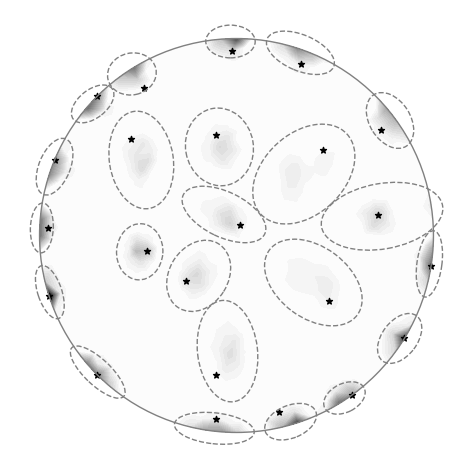
\includegraphics[scale=0.33]{batch1.png}
		%		\caption{Non-symmetric}
	\end{subfigure}
	\begin{subfigure}{0.32\textwidth}
		\centering
		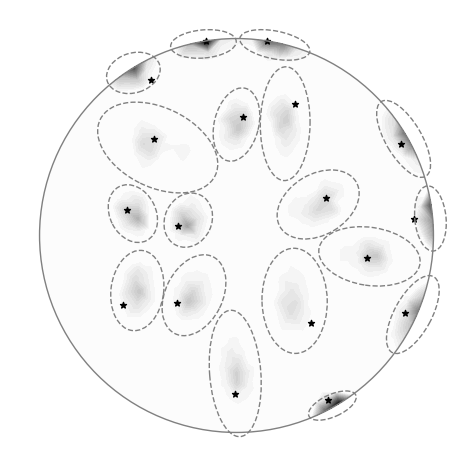
\includegraphics[scale=0.33]{batch12.png}
		%		\caption{Non-symmetric}
	\end{subfigure}
	\begin{subfigure}{0.32\textwidth}
		\centering
		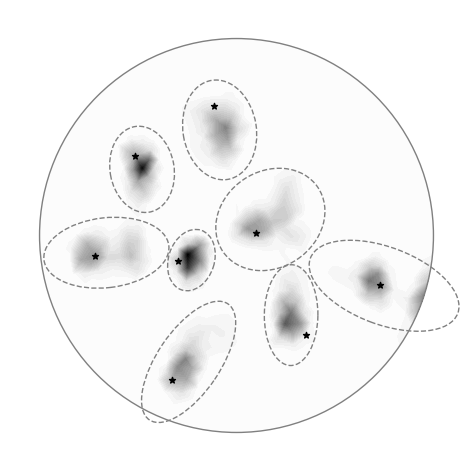
\includegraphics[scale=0.33]{batch19.png}
		%		\caption{Non-symmetric}
	\end{subfigure}
	\caption{Batches, $\eta_b$, of normalized impulse responses, $\phi_{x_i}/V(x_i)$, for the Stokes inverse problem Hessian. Left: 2nd batch. Mid: 13th batch. Right: 19th batch. Brightness scale differs between the subfigures. Black stars indicate the sample point locations, $x_i$. Dashed gray ellipses indicate the support ellipsoids, $E_{x_i}$. The large circle is the boundary of the domain $\Omega$. Early batches tend to have lots of ellipsoids near the boundary, as compared to later batches. This is because our greedy ellipsoid packing algorithm tries to pick sample points that are far away from sample points in previously chosen batches.}
	\label{fig:batches_intro}
\end{figure}

The output of our method is a hierarchical matrix (H-matrix) approximation, $\mathbf{A}_H$, of a discretization of $\Aop$. H-matrices are a matrix format in which the rows and columns of the matrix are re-ordered, then the matrix is recursively subdivided into blocks, in such a way that many off-diagonal blocks are low rank. For more details about H-matrices, see Appendix \ref{app:h_matrix}. While operator actions of $\Aop$ on vectors are typically computationally expensive, fast H-matrix methods permit us to perform matrix-vector products with $\mathbf{A}_H$ cheaply. Furthermore, one may use H-matrix methods to perform useful linear algebra operations involving $\mathbf{A}_H$ that cannot easily be done using $\Aop$, because $\Aop$ is only available matrix-free. These operations include matrix-matrix addition, matrix-matrix multiplication, matrix factorization, and matrix inversion. These H-matrix methods are fast and scale well to large problems. The ability to perform these operations permits, for example, fast solution of Newton linear systems in PDE-constrained optimization, fast sampling of ill-conditioned posterior distribution in Bayesian inverse problems, and construction of high rank surrogate models that can be used for uncertainty quantification.


%
% Because we build a H-matrix, and 
%
%In this paper we form hierarchical matrix approximations, $\mathbf{A}_H$, of operators $\Aop$ that satisfy the following three properties:
%\begin{description}
%	\item[Locally supported impulse responses:] For all $x\in \Omega$, the support of $\impulseresponse_x$ is contained (or approximately contained) in a localized region.
%	\item[Non-negative impulse responses:] We have
%	\begin{equation*}
%	\impulseresponse_x(y) \ge 0
%	\end{equation*}
%	for all (or approximately all) $(y,x) \in \Omega \times \Omega$.
%%	\item[Matrix-free:] One cannot easily evaluate kernel entries $\Aker(y,x)$. Instead, access to $\Aop$ is available through ``operator actions.'' That is, we have a black-box computational procedure (which is typically expensive) through which we may evaluate the maps
%%	\begin{equation*}
%%	u \mapsto\Aop u \quad \text{and} \quad v \mapsto \Aop^Tv
%%	\end{equation*} 
%%	for arbitrary functions $u$ and $v$. After discretization (see Appendix \ref{app:discretized_operations}), $\Aop$ becomes a dense matrix, $\bm{A}$, that is typically too large to be built and stored. This property is called ``matrix-free'' because at the discrete level it means that one can perform matrix-vector products of $\bm{A}$ and $\bm{A}^T$ with arbitrary vectors, but one cannot easily\footnote{One could compute $\bm{v} = \bm{A}\bm{e}_j$, where $\bm{e}_j=(0,\dots,0,1,0,\dots,0)$ is the unit vector which has $j^\text{th}$ component equal to one and all other components equal to zero, then extract $\bm{A}_{ij} = \bm{v}_i$. However, this process is wasteful because one computes the entire vector $\bm{v}$, then discards all but one component.} access matrix entries $\bm{A}_{ij}$. In applications, applying $\bm{A}$ to a vector may involve iteratively solving a large linear system, timestepping, or performing some other nontrivial computational procedure. 
%%	%For example, in reduced space approaches to PDE-constrained optimization and inverse problems, Hessian information is available only through the application of the Hessian to vectors, and one such Hessian application requires solving two PDEs \cite{HESSIANADJOINT}. 
%\end{description} 
%Once the hierarchical matrix approximation $\mathbf{A}_H$ is constructed, one may use H-matrix methods to perform further useful linear algebra operations involving $\mathbf{A}_H$, including matrix-matrix addition, matrix-matrix multiplication, matrix-vector products, matrix factorization, and matrix inversion. These H-matrix methods are fast and scale well to large problems. WHY DO THESE OPERATIONS: KRYLOV SOLVERS, SAMPLING STRATEGIES, CAN'T DO WITH A.
%
%% approximate operators which possess the following properties:
%% 
%%We further limit our focus to operators that have
%%\textbf{Local support}
%%We say that $\Aop$ has local support if, for all $x\in \Omega$, the support of $\impulseresponse_x$ is contained (or approximately contained) in a small region. 
%%The smaller these supports are, the better our algorithm will perform.  Let $\delta_x$ denote the delta distribution (point source) centered at $x$. From \eqref{eq:impulse_response_delta_action}, we see that this local support property means that the response of $\Aop$ to a point source at $x$ is zero (or small) at points $y$ that are far from $x$.
%%\item[3) Local translation invariance:] We say that $\Aop$ is locally translation invariant if
%%\begin{equation}
%%	\label{eq:local_translation_invariance}
%%	\Aker(y+h, x+h) \approx \Aker(y,x)
%%\end{equation}
%%when $h$ is not too large. One can imagine the kernel entry $\Aker(y,x)$ as representing the strength of an interaction between a source at point $x$ and a target at point $y$. Local translation invariance means that the interaction strength remains roughly the same if the source and target points are both translated by the same vector. This is illustrated in Figure FIG.
%%\textbf{Non-negative impulse response:} We have
%%\begin{equation*}
%%\impulseresponse_x(y) \ge 0
%%\end{equation*}
%%for all $(y,x) \in \Omega \times \Omega$.



\subsection{Motivation: PDE constrained inverse problems}
\label{sec:PDE_hessian_motivation}

Our motivation for this work is approximation of Hessians in distributed parameter inverse problems governed by partial differential equations (PDEs). That is, inverse problems in which one seeks to reconstruct an unknown parameter field, $m$, from noisy observations, 
\begin{equation*}
	y = f(m, u(m)) + \text{noise},
\end{equation*}
which depend on  a state variable $u$. In turn, $u$ depends on $m$ implicitly through the solution of a PDE, which we write generically as follows:
\begin{equation}
	\label{eq:state_pde}
	0 = g(m,u).
\end{equation}
Here $u(m)$ denotes the solution of the PDE \eqref{eq:state_pde} as a function of $m$. In the deterministic approach to inverse problems, one typically finds $m$ as the solution to the minimization problem 
\begin{equation}
	\label{eq:minimization_problem}
	\min_m \quad \frac{1}{2}\|y - f(m,u(m))\|_W^2 + \mathcal{R}(m),
\end{equation}
where $\|\cdot\|_W$ is weighted norm which depends on the noise covariance, and $\mathcal{R}(m)$ is a regularization term. The objective function in optimization problem \eqref{eq:minimization_problem} is defined indirectly via the implicit function theorem. As a result, information about the Hessian of the objective function, $\mathcal{H}$, is only accessible via the action of $\mathcal{H}$ action on vectors. In particular, applying $\mathcal{H}$ to a vector requires solving two PDEs \cite{HESSIANACTION}. More accessible approximations of $\mathcal{H}$ are highly desirable, because they allow for fast solution of \eqref{eq:minimization_problem} via Newton-type methods. More accessible Hessian approximations are also central to many methods for uncertainty quantification in Bayesian statistical approaches to the inverse problem, because $\mathcal{H}^{-1}$ locally approximates the Bayesian posterior covariance for $m$. 


\subsection{Background}

The most popular matrix-free operator approximation methods are based on low rank approximation \cite{CCGOPAPERS}. This includes the Lanczos method, the randomized singular value decomposition \cite{HMTRANDOM}, and CUR approximation/skeletonization \cite{CUR,MAHONEY}. However, low rank approximation is not suitable for high rank operators, and many operators of practical interest are high rank. In the context of Hessians, methods based on low rank approximation suffer from a ``data predicament''---if the data are highly informative about the unknown parameter, then the numerical rank of the data misfit term in the Hessian is large, so a large number of operator actions are required to form an accurate ``low rank'' approximation \cite{MYDISSERTATION}. 
%The ideal scenario from a scientific perspective (highly informative data) is therefore the worst case scenario from a computational perspective (large computational cost) \cite{MYDISSERTATION}. 


%In general, product-convolution approximations take the form shown in \eqref{eq:product_convolution}, but $\convkernel_i$ and $w_i$ may be arbitrary functions.
Product-convolution (PC) approximations are approximations of an operator by weighted sums of convolution operators with spatially varying weights. A single convolution operator may be high rank, so PC approximations can (where applicable) approximate high rank operators efficiently. PC approximations have been used in a variety of fields going back several decades \cite{PRODCONVLIST}. Often PC methods are known as ``point spread function'' (PSF) methods, particularly in optics and image processing. There, the ``operator'' $\Aop$ is a physical process of distortion and blurring of light rays passing through an optical system such as a telescope or microscope. However, ``PSF'' is sometimes used as an umbrella term to refer to other approximation methods that focus on interpolating impulse responses or impulse response features.
%, including CUR-based low rank approximation \cite{NAGYPSFCUR}.
For background on PC and PSF methods, we recommend the following papers: \cite{PRODCONVGOOD}. 

Our method is not a PC approximation, but it builds upon a class of PC approximations in which the convolution kernels are shifted impulse responses of $\Aop$ associated with a collection of points $x_i \in \Omega$ \cite{PRODCONVLIST}. A popular choice for PC methods in this class is to choose the $x_i$ to be nodes in a regular grid \cite{NAGY}.
%, and interpolate the convolution operators with piecewise linear interpolation \cite{NAGY}, splines \cite{PRODCONVSPLINES}, or radial basis functions \cite{PRODCONVRBF}. 
With a regular grid, a large number of $x_i$ are typically required to achieve an accurate approximation. In our previous work, we reduced the computational cost by starting with a coarse grid of points $x_i$, then adaptively refining the grid in the regions where the error in the approximation is large \cite{PRODCONVMYPAPER}. But even with adaptive refinement, many $x_i$, and hence operator actions of $\Aop$, are required. 

In this paper, 
%rather than using adaptive refinement, 
we reduce the computational cost by picking points $x_i$ in a way that allows many $\phi_{x_i}$ to be computed with each operator action of $\Aop$. This requires us to estimate the supports of the $\phi_x$, \emph{before} we compute them. We were inspired by techniques from resolution analysis in seismic imaging \cite{RESOLUTION}. In resolution analysis, $\Aop$ is the Hessian for a seismic inverse problem, and the width of $\phi_x$ is used to estimate of the minimum length scale on which features of the parameter can be inferred near the point $x$. If the width of $\phi_x$ is ten meters, then features of the parameter near $x$ can be accurately inferred from data if those features are larger than roughly ten meters in size. In \cite{RESOLUTION}, the width of $\phi_x$ is estimated to be the local autocorrelation length of the function $\Aop^T \zeta$ near $x$, where $\zeta$ is a random noise funtion. Rather than probing $\Aop^T$ with random noise functions, we use polynomial functions (see Sections \ref{sec:intromoments} and \ref{eq:mean_and_covariance_estimation}). Our method estimates the support of $\phi_x$ more accurately and reliably than random noise probing, but our method requires that $\Aop$ has a positive integral kernel, while random noise probing does not have this requirement.
%(and moreover, the seismic Hessian does not have a non-negative integral kernel).

Convolutions can be performed using the fast Fourier transform (FFT) \cite{PRODCONVFFT}, which allows PC approximations to be used as a fast surrogates for $\Aop$. Often it is necessary to perform further linear algebra operations involving $\Aop$, such as solving linear systems with $\Aop$ as the coefficient operator. Conventionally, one performs these linear algebra operations using Krylov methods, replacing $\Aop$ with its PC approximation \cite{PRODCONVKRYLOV}. The Krylov method is accelerated because performing matrix vector products with the product-convolution approximation is typically faster than performing operator actions with $\Aop$. However, there are several problems with this approach. First, the number of Krylov iterations can be large, particularly when $\Aop$ is high-rank. Second, complicated geometries are rarely discretized using regular grids, so using the FFT to perform convolutions requires transferring discretized functions back and forth between the irregular mesh and a regular grid. Third, the computational cost grows with the number of convolution kernels used. 
%If a large number of convolution kernels are used, this approach can be slow.
%Furthermore, in big-data inverse problems the required number of Krylov iterations is large \cite{MYDISSERTATION,OTHERS}. 
Thus, 
%after constructing the product-convolution approximation, 
it is desirable to convert the PC approximation to other matrix formats that are amenable to faster linear algebra operations. Wavelet compression methods have been used for this purpose \cite{PRODCONVWAVELETS}, because operators that are amenable to PC approximation are often sparse in the wavelet domain. Convolution-product approximations (transposes of PC approximations) are equivalent to low rank approximation of the pseudo-differential symbol of the operator, so one could perform linear algebra operations involving PC approximations using fast methods for pseudo-differential operator symbol calculus \cite{YINGDEMANET}. Other matrix-free operator approximation methods based on wavelets \cite{HERRMANN} and pseudo-differential operators \cite{DEMANET} do not use PC approximation. Here, we follow our previous work \cite{PRODCONVMYPAPER}, in which we converted PC approximations into H-matrix format. 

Since our end goal is constructing an H-matrix, we are freed from strict adherence to the PC format. This allows us to modify the PC approach to address well-known deficiencies. PC approximations are based on an assumption of local translation invariance \cite{LOCATRANSLATIONINVARIANCE}, while our method is based on an assumption that we call ``normalized local mean displacement invariance,'' which is more general than local translation invariance, and includes both low rank approximation and local translation invariance as special cases (see Section \ref{sec:local_mean_displacement_invariance}). PC approximations have well-known issues near boundaries called boundary artifacts, which are caused by the boundary artificially ``cutting off'' impulse responses. 
%One must extend the impulse responses outside of the domain where they are undefined, but
%. Various extension techniques have been used, such as extension by zero, and reflection across the boundary, yet 
%no known extension technique is fully satisfactory \cite{BOUNDARYETENSION}. 
In our method we do not have an issue with boundary artifacts because we temporarily exclude impulse responses from the approximation procedure whenever the approximation procedure attempts to evaluate the impulse response at a location where it is undefined. Our approximation cannot be written as a weighted sum of convolution operators, so we cannot apply our approximation to vectors via the FFT. This is fine because our approximation is an H-matrix, which can be applied to vectors even faster.

%MOMENTS PERMIT IMPROVED INTERPOLATION. IMPROVED INTERPOLATION REQUIRES H-MATRIX. H-MATRIX WITH IMPROVED INTERPOLATION ALSO SOLVES BOUNDARY ARTIFACT PROBLEM. ALSO DOESNT REQUIRE REGULAR GRID. ALSO SCALABLE TO LARGE NUMBER OF IMPULSE RESPONSES. FFT HAS FAST MATVEC BUT NOT OTHER OPTIONS.



Since we are building an H-matrix approximation of $\Aop$, it is natural to ask why we need to compute impulse responses and interpolate them. Why not build the H-matrix directly?
%Can we build the H-matrix directly? In short, no, not efficiently. 
The reason is that classical H-matrix construction methods \cite{HMATRIXCONSTRUCTION} require access to matrix entries of the matrix being approximated, and therefore cannot be used to efficiently form H-matrix approximations of operators that are only available through matrix-vector products. Our impulse response interpolation lets us quickly compute approximations to matrix entries, which allows us to use these classical H-matrix construction methods. There are newer matrix-free methods for H-matrix approximation based on the so-called ``peeling process'' \cite{LEXINGPEELINGPROCESS}, and these methods have been used to form H-matrix representations of Hessians in PDE constrained inverse problems \cite{ILONAHMATRIX,NOEMIHMATRIX}. While these matrix-free H-matrix construction methods are asymptotically scalable in theory, in practice the required number of matrix vector products is unreasonably large. Matrix-free H-matrix construction methods are currently a topic of considerable research, so future algorithmic improvements may make matrix-free H-matrix methods more feasible in the future. 


%Product-convolution type approximations of Hessians have been used in a seismic inverse problem in \cite{GEORGSEISMICPRODCONV}, and in an advection-diffusion inverse problem in \cite{PRODCONVMYPAPER}. In \cite{DEMANETSEISMIC}, matrix probing \cite{MATRIXPROBING} is used to approximate the Hessian in a seismic inverse problem as the sum of simple pseudodifferential operators. Although it is not explicitly mentioned, the approximation in \cite{DEMANETSEISMIC} could be interpreted as a convolution-product approximation (a product-convolution approximation of the transpose of the operator).
%, which is like a product-convolution approximation, except the order of pointwise multiplications and convolutions is reversed in \eqref{eq:product_convolution}.

\section{Main concepts}
\label{sec:prerequisites}

In this section we present three main concepts that our method is based on. The method itself will be presented in Section \ref{sec:method}. First, we define moments of the impulse responses, $\phi_x$, and show how these moments can be computed efficiently (Section \ref{sec:intromoments}). Our method will use these moments extensively. Second, we present ellipsoid shaped a-priori estimates for the supports of the impulse responses (Section \ref{eq:mean_and_covariance_estimation}). Our method will use these ellipsoid estimates to choose sets of impulse responses that can be computed in batches. Third, we describe a method of approximating impulse responses by other nearby impulse responses, which we call ``normalized local mean displacement invariance'' (Section \ref{sec:local_mean_displacement_invariance}). Our method will interpolate impulse responses using this approximation. 



\subsection{Impulse response moments}
\label{sec:intromoments}

The impulse response $\impulseresponse_x$ may be interpreted as a scaled probability distribution because of the non-negative integral kernel property. Let $\spatialvol:\Omega \rightarrow \mathbb{R}$,
\begin{equation*}
\spatialvol(x) := \int_\Omega \impulseresponse_x(y) dy
\end{equation*}
denote the spatially varying scaling factor,
%, let 
%\begin{equation}
%\label{eq:scaled_impulse_response}
%\widehat{\impulseresponse}_x := \impulseresponse_x / \spatialvol(x)
%\end{equation}
%denote the normalized version of $\impulseresponse_x$. 
and let $\mu:\Omega \rightarrow \mathbb{R}^d$, $\Sigma:\Omega \rightarrow \mathbb{R}^{d \times d},$
\begin{equation*}
\spatialmean(x) := \mathbb{E}(\impulseresponse_x / V(x)), \qquad
\spatialcov(x) := \Var(\impulseresponse_x /V(x)),
\end{equation*}
to be the spatially varying mean and covariance of the normalized version of $\impulseresponse_x$, respectively. Imagine $\phi_x$ as a mound of dirt piled on a localized region in $\Omega$, with $\phi_x(y)$ being the height of the dirt mound at location $y$. The scalar $V(x)$ is the total volume of dirt in the mound, the vector $\mu(x)$ is the center of mass of the dirt mound, and the matrix $\Sigma(x)$ contains information about how wide the dirt mound is in each spatial direction. 

%The ellipsoid $E_x$ is not immediately available. 
%(recall $\gdim$ is the spatial dimension of $\Omega$).
The direct approach to compute $\spatialvol(x)$, $\spatialmean(x)$, and $\spatialcov(x)$ is to apply $\Aop$ to a point source centered at $x$ to get $\impulseresponse_x$, as per \eqref{eq:impulse_response_delta_action}. Then one can post-process $\impulseresponse_x$ to determine $\spatialvol(x)$, $\spatialmean(x)$, and $\spatialcov(x)$. But this direct approach is computationally infeasible because it requires one operator action of $\Aop$ per point $x$, and our method will need to know $V(x)$, $\mu(x)$, and $\Sigma(x)$ at all points $x$. Fortunately, it is possible to compute $\spatialvol(x)$, $\spatialmean(x)$, and $\spatialcov(x)$, \emph{for all points $x\in\Omega$ simultaneously}, by applying $\Aop^T$ to one constant function, $\gdim$ linear functions, and $\gdim(\gdim+1)/2$ quadratic functions. Specifically, let  $x^i$ denote the $i^\text{th}$ component of $x$, i.e., $x = \left(x^1, x^2, \dots, x^\gdim\right)$, and let $C$, $\{L^i\}_{i=1}^\gdim$, and ${\{Q^{ij}\}_{i=1}^\gdim}_{j=1}^\gdim$ be the following constant, linear, and quadratic functions:
\begin{equation*}
C(x) := 1, \qquad
L^i(x) := x^i, \qquad
Q^{ij}(x) = x^i x^j.
\end{equation*}
The following results (derived in Appendix \ref{app:proofs}) follow straightforwardly from the definitions:
\begin{subequations}
	\label{eq:vol_mean_var}
	\begin{align}
	\spatialvol =& \left(\Aop^T C\right)^* \\
	\spatialmean^i =& \left(\Aop^T L^i\right)^* / \spatialvol \\
	\spatialcov^{ij} =& \left(\Aop^T Q^{ij}\right)^* / \spatialvol - \spatialmean^i\cdot \spatialmean^j
	\end{align}
\end{subequations}
for $i=1,\dots, \gdim$, $j=1,\dots,\gdim$. Here $f/g$ denotes pointwise division of functions, $\left(f/g\right)(x) = f(x)/g(x)$, and $f\cdot g$ denotes pointwise multiplication of functions, $(f\cdot g)(x) = f(x)g(x)$. The resulting method form computing $V$, $\mu$, and $\Sigma$ is shown in Algorithm \ref{alg:varhpi_mean_cov}.

\begin{algorithm2e}
	\SetAlgoNoLine
	\SetKwInOut{Input}{Input}
	\SetKwInOut{Output}{Output}
	{	
		\Input{Operator $\Aop$}
		\Output{$\spatialvol$, $\spatialmean$, and $\spatialcov$}
		
		\tcp{Compute scaling factor $\spatialvol$}
		
		Form constant function $C(x)=1$
		
		Compute $\spatialvol = \left(\Aop^T C\right)^*$
		
		\tcp{Compute mean $\spatialmean$}
		\For{$i=1,2,\dots,\gdim$}{
			Form linear function $L^i(x) = x^i$
			
			Compute $\spatialmean^i = \left(\Aop^T L^i\right)^* / \spatialvol$
		}
		\tcp{Compute covariance $\spatialcov$}
		\For{$i=1,2,\dots,\gdim$}{
			\For{$j=1,\dots,i$}{
				Form quadratic function $Q^{ij}(x) = x^i x^j$
				
				Compute $\spatialcov^{ij} = \left(\Aop^T Q^{ij}\right)^* / \spatialvol - \spatialmean^i\cdot \spatialmean^j$
				
				Set $\spatialcov^{ji} = \spatialcov^{ij}$
				
			}
		}
		
	}
	\caption{Compute scaling factor $\spatialvol$, mean $\spatialmean$, and covariance $\spatialcov$}
	\label{alg:varhpi_mean_cov}
\end{algorithm2e}

%We present this efficient method of computing $\spatialvol$, $\spatialmean$, and $\spatialcov$ in Proposition \ref{thm:vol_mean_cov} and summarize the method for computing these moments in Algorithm \ref{alg:varhpi_mean_cov}.


%\begin{prop}[Impulse response moments]
%	\label{thm:vol_mean_cov}
%	%	Let $\spatialvol:\Omega \rightarrow \mathbb{R}$, $\spatialmean:\Omega \rightarrow \mathbb{R}^\gdim$, and $\spatialcov:\Omega \rightarrow \mathbb{R}^{\gdim \times \gdim}$, be the following functions:
%	%	\begin{equation*}
%	%	\spatialvol(x) := \int_{\Omega} \impulseresponse_x(y) dy, \qquad
%	%	\spatialmean(x) := \mathbb{E}(\widehat{\impulseresponse}_x), \qquad
%	%	\spatialcov(x) := \Var(\widehat{\impulseresponse}_x),
%	%	\end{equation*}
%	%	where $\widehat{\impulseresponse}_x := \impulseresponse_x / \spatialvol(x)$ denotes the normalized version of $\impulseresponse_x$, $\mathbb{E}(\widehat{\impulseresponse}_x)$ denotes the mean of $\widehat{\impulseresponse}_x$, and $\Var(\widehat{\impulseresponse}_x)$ denotes the variance of $\widehat{\impulseresponse}_x$.	
%	Let  $x^i$ denote the $i^\text{th}$ component of $x$, i.e., $x = \left(x^1, x^2, \dots, x^\gdim\right)$. Let $C$, $\{L^i\}_{i=1}^\gdim$, and ${\{Q^{ij}\}_{i=1}^\gdim}_{j=1}^\gdim$ be the following constant, linear, and quadratic functions:
%	\begin{equation*}
%	C(x) := 1, \qquad
%	L^i(x) := x^i, \qquad
%	Q^{ij}(x) = x^i x^j.
%	\end{equation*}
%	Let $f/g$ denote the pointwise division of functions, $\left(f/g\right)(x) = f(x)/g(x)$, and $f\cdot g$ denote the pointwise multiplication of functions, $(f\cdot g)(x) = f(x)g(x)$. The following results hold:
%	\begin{subequations}
%		\label{eq:vol_mean_var}
%		\begin{align}
%		\spatialvol =& \left(\Aop^T C\right)^* \\
%		\spatialmean^i =& \left(\Aop^T L^i\right)^* / \spatialvol \\
%		\spatialcov^{ij} =& \left(\Aop^T Q^{ij}\right)^* / \spatialvol - \spatialmean^i\cdot \spatialmean^j
%		\end{align}
%	\end{subequations}
%	for $i=1,\dots, \gdim$, $j=1,\dots,\gdim$.
%\end{prop}

%The proof of Proposition \ref{thm:vol_mean_cov} is shown in Appendix \ref{app:proofs}. The proof is straightforward, and follows directly from the definitions.


\subsection{Impulse response support ellipsoids}
\label{eq:mean_and_covariance_estimation}

%Because of the non-negative impulse response property, for each $x \in \Omega$, the impulse response $\impulseresponse_x$ is a non-negative function $y \mapsto \impulseresponse_x(y)$. Hence, $\impulseresponse_x$ is a scaled probability distribution. Let $\spatialvol(x) := \int_\Omega \impulseresponse_x(y) dy$ denote the scaling factor (the ``volume'' of $\impulseresponse_x$), let $\widehat{\impulseresponse}_x := \impulseresponse_x / \spatialvol(x)$ denote the normalized version of $\impulseresponse_x$, and let $\spatialmean(x)$ and $\spatialcov(x)$ denote the mean and covariance of $\widehat{\impulseresponse}_x$, respectively. 

We make the approximation that the support of $\impulseresponse_x$ is contained within the ellipsoid
\begin{equation}
\label{eq:support_ellipsoid}
E_x := \{x' \in \Omega: (x' - \spatialmean(x))^T \spatialcov(x)^{-1} (x' - \spatialmean(x)) \le \tau^2\},
\end{equation}
where $\tau$ is a fixed constant. The ellipsoid $E_x$ is the set of points within $\tau$ standard deviations from the mean of the Gaussian distribution with mean $\spatialmean(x)$ and covariance $\spatialcov(x)$, i.e., the Gaussian distribution which has the same mean and covariance as the normalized version of $\impulseresponse_x$.

The quantity $\tau$ is a parameter that must be chosen by the user. The larger $\tau$ is, the larger the ellipsoid $E_x$ is, and the more conservative the estimate is for the support of $\impulseresponse_x$. However, in Section \ref{sec:sample_point_selection} we will see that the cost of our algorithm depends on how many non-overlapping ellipsoids $E_x$ we can ``pack'' in the domain $\Omega$ (more ellipsoids $\implies$ lower cost), and choosing a larger value of $\tau$ means that fewer ellipsoids will fit in $\Omega$. We find that $\tau=3$ yields a reasonable balance between these competing interests, and use $\tau=3$ in our numerical results. The fraction of the ``mass'' of $\impulseresponse_x$ residing outside of $E_x$ is less than $1/\tau^2$ by Chebyshev's inequality, though this bound is conservative and typically far less mass resides in this region. 

%To determine $E_x$, we must compute the scalar $\spatialvol(x)$, the length-$\gdim$ vector $\spatialmean(x)$, and the $\gdim \times \gdim$ matrix $\spatialcov(x)$. In Section \ref{eq:mean_and_covariance_estimation} we will see that it is possible to compute $V(x)$, $\mu(x)$, and $\Sigma(x)$ for all $x \in \Omega$ simultaneously, via a procedure that involves applying $\Aop^T$ to a small number of polynomial functions (three functions if $\gdim=1$, six if $\gdim=2$, ten if $\gdim=3$).




\subsection{Local mean-displacement invariance}
\label{sec:local_mean_displacement_invariance}

Let $x$ and $x'$ be points in $\Omega$ that are ``close'' to each other, and consider the following four approximations, ordered by increasing level of sophistication:
\begin{align}
\phi_x(y) &\approx \phi_{x'}(y) \label{eq:translate1}\\
\phi_x(y) &\approx \phi_{x'}(y-x+x') \label{eq:translate2}\\
\phi_x(y) &\approx \phi_{x'}\left(y-\mu(x)+\mu(x')\right) \label{eq:translate3}\\
\phi_x(y)/V(x) &\approx \phi_{x'}\left(y-\mu(x)+\mu(x')\right) / V(x'). \label{eq:translate4}
%\frac{\phi_x(y)}{V(x)} &\approx \frac{\phi_{x'}\left(y-\mu(x)+\mu(x')\right)}{V(x')}. \label{eq:translate4}
\end{align}
Approximation \eqref{eq:translate1} says that $\phi_x$ can be approximated by $\phi_{x'}$ when $x$ and $x'$ are close. 
%This approximation follows from the assumption that $\Phi$ is smooth. 
Operators satisfying \eqref{eq:translate1} can be well-approximated via low-rank interpolative factorization/Nystrom approximation \cite{CUR,NYSTROM}.
% of the form
%\begin{equation}
%	\label{eq:low_rank_interpolation}
%	\Phi(y,x) \approx \sum_{i=1}^r w_i(x) \phi_{x_i}(y)
%\end{equation}
%where $\phi_{x_i}$ are known impulse responses at a collection of points $x_i$ scattered throughout $\Omega$, and $w_i$ are smooth weighting functions that interpolate the $\phi_{x_i}$. 
%In problems of practical interest, \eqref{eq:translate1} typically holds \emph{asymptotically} in the limit as $x'$ approaches $x$. 
However, 
%even if $\Phi$ is smooth (which is typically the case asymptotically),
%the relevant Lipschitz constant for continuity, and hence 
the required rank in the low rank approximation can be large, which makes algorithms based on \eqref{eq:translate1} computationally expensive. This is the case for Hessians in PDE constrained inverse problems with highly informative data, as discussed in Section \ref{sec:PDE_hessian_motivation}. 
%As the data become more informative, typically the ``mass'' of $\Phi(y,x)$ concentrates nearer and nearer to the ``diagonal'' $y=x$, the Lipschitz constant increases, and the required rank in the approximation increases.
%Moreover, if $\Aop$ is numerically low rank, then one would typically use more accurate and robust matrix-free methods for forming low-rank approximations, such as randomized SVD or Lanczos.

Operators that satisfy \eqref{eq:translate2} are called ``locally translation-invariant'' because integral kernel entries $\Phi(y,x)$ for such operators are approximately invariant under translation of $x$ and $y$ by the same displacement, i.e., $x \rightarrow x+h$ and $y \rightarrow y+h$. Locally translation-invariant operators act like convolutions locally, and can therefore be well-approximated by so-called product-convolution approximations---weighted sums of convolution operators with spatially varying weights. Product-convolution approximations can be high-rank even if the number of convolution operators used in the approximation is small.

% Kernels for locally translation invariant operators can be well-approximated by decompositions of the form
%\begin{equation}
%	\Phi(y,x) \approx \sum_{i=1}^r w_i(x) \phi_{x_i}(y-x)
%\end{equation}
%which correspond to operator approximations of the form
%\begin{equation}
%\label{eq:product_convolution}
%\left(\Aop~u\right)(v) \approx \left( v,~ \sum_{i=1}^\convrank \convkernel_i \ast \left(w_i \cdot u\right) \right)_{L^2(\Omega)}.
%\end{equation}
%Here $f \ast g$ denotes convolution, and $f \cdot g$ denotes pointwise multiplication of the functions $f$ and $g$ (i.e., $\left(f \cdot g\right)(x) = f(x) g(x)$). Approximations of the form \eqref{eq:product_convolution} are known as \emph{product-convolution} approximations, because the action of each term in the sum consists of a pointwise product, followed by a convolution. Product-convolution approximations can be high-rank even if $r$ is small.

\begin{figure}
	\begin{center}
		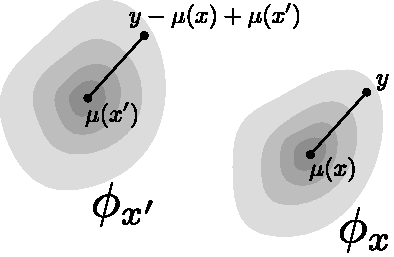
\includegraphics[scale=1.0]{mean_displacement_invariance.pdf}
	\end{center}
	\caption{An operator is locally mean-displacement invariant if $\impulseresponse_{x}(y) \approx \impulseresponse_{x'}\left(y - \mu(x) + \mu(x')\right)$ when $x$ is close to $x'$.}
	\label{fig:mean_displacement_invariance}
\end{figure}


Approximation \eqref{eq:translate3} improves upon \eqref{eq:translate1} and \eqref{eq:translate2}, and generalizes both. On one hand, if \eqref{eq:translate1} holds, then $\mu(x) \approx \mu(x')$, and so \eqref{eq:translate3} holds. On the other hand, translating a distribution translates its mean, so if \eqref{eq:translate2} holds, then $\mu(x')-\mu(x) \approx x' - x$, so again \eqref{eq:translate3} holds. But approximation \eqref{eq:translate3} can hold in situations where neither \eqref{eq:translate1} nor \eqref{eq:translate2} holds. For example, because the expected value commutes with affine transformations, \eqref{eq:translate3} will hold when an $\Aop$ is locally translation-invariant with respect to a rotated frame of reference, while \eqref{eq:translate2} will not hold in this case. Additionally, \eqref{eq:translate3} generalizes to operators $\Aop:L^2(\Omega_1) \rightarrow L^2(\Omega_2)'$ that map between function spaces on different domains $\Omega_1$ and $\Omega_2$, and even operators that map between domains with different spatial dimensions. In contrast, \eqref{eq:translate2} does not naturally generalize to operators that map between function spaces on different domains, because the formula $y-x+x'$ requires vectors in $\Omega_2$ and $\Omega_1$ to be added together.  We call \eqref{eq:translate3} ``local mean-displacement invariance,'' and illustrate \eqref{eq:translate3} in Figure \ref{fig:mean_displacement_invariance}.

We use approximation \eqref{eq:translate4}, which is the same as \eqref{eq:translate3}, except for the extra factors of $1/V(x)$ on the left hand side and $1/V(x')$ on the right hand side. These factors make the approximation more robust if $V(x)$ varies widely. Approximation \eqref{eq:translate4} is equivalent to \eqref{eq:translate3}, but with $\phi_x$ replaced by the its normalized version, $\phi_x/V(x)$. We call \eqref{eq:translate4} ``normalized local mean-displacement invariance.''



\section{Method}
\label{sec:method}

After discretization with finite elements\footnote{While we use finite elements, other discretization schemes such as finite differences or finite volumes could be used instead, with minor modifications to our method.} (Section \ref{sec:finite_element_kernel}), $\Aop$ and $\Phi$ become large dense matrices $\mathbf{A}$ and $\mathbf{\Phi}$, respectively. Because $\Aop$ is only available matrix-free and $\Phi$ is only defined implicitly in terms of $\Aop$, the matrices $\mathbf{A}$ and $\mathbf{\Phi}$ are not easily accessible. Directly computing and storing these matrices is computationally intractible. In this section, we present our method for constructing accessible H-matrix approximations, $\mathbf{A}_H$ and $\mathbf{\Phi}_H$ of $\mathbf{A}$ and $\mathbf{\Phi}$, respectively, using a small number of operator actions of $\Aop$ and $\Aop^T$. 

%Fourth, we discuss how discretization of continuous functions by finite elements leads to matrix discretizations $\mathbf{A}$ and $\mathbf{\Phi}$ of $\Aop$ and $\Phi$, respectively (Section \ref{sec:finite_element_kernel}). The primary function of our method is to compute H-matrix approximations of these matrices. 
%While we use finite elements, other discretization schemes such as finite differences or finite volumes could be used instead with minor modifications.

\subsection{Overview}
\label{sec:method_overview}

Algorithm \ref{alg:varhpi_mean_cov} from Section \ref{sec:intromoments} allows us to compute $V$, $\mu$, and $\Sigma$ by applying $\Aop^T$ to a small number of polynomial functions, and \eqref{eq:support_ellipsoid} from Section \ref{eq:mean_and_covariance_estimation} uses $V$, $\mu$, and $\Sigma$ to form an ellipsoid shaped estimate for the support of $\phi_x$, \emph{without} computing $\phi_x$. This allows us to compute large numbers of impulse responses, $\impulseresponse_{x_i}$, in ``batches,'' $\eta_b$ (see Figure \ref{fig:batches_intro}). We compute the impulse response batch $\eta_b$ by applying $\Aop$ to a weighted sum of point sources (Dirac comb) associated with a batch, $S_b$, of points $x_i$ scattered throughout $\Omega$ (Section \ref{sec:get_impulse_response}). The batch of points $S_b$ is chosen via a greedy ellipsoid packing algorithm so that, for $x_i,x_j \in S_b$, the support of $\impulseresponse_{x_i}$ and the support of $\impulseresponse_{x_j}$ do not overlap (or do not overlap much) if $i \neq j$ (Section \ref{sec:sample_point_selection}). Because these supports do not overlap, we can post-process $\eta_b$ to recover the functions $\impulseresponse_{x_i}$ associated with all points $x_i \in S_b$---with one application of $\Aop$, we recover many $\impulseresponse_{x_i}$ (Section \ref{sec:get_impulse_response}). The process is repeated to get more batches, until a desired number of impulse responses is reached.

Once the impulse response batches $\eta_b$ are computed, we approximate the integral kernel $\Phi(y,x)$ at arbitrary points $(y,x)$ by interpolation (Section \ref{sec:approximate_kernel_entries}). The key idea behind the interpolation is the normalized local mean displacement invariance assumption discussed in Section \ref{sec:local_mean_displacement_invariance}.
%Specifically, we make the assumption that
%\begin{equation}
%\Phi(y,x) = \phi_x(y) \approx \phi_{x_i}(y - \mu(x) + \mu(x_i))
%\end{equation}
%if $x_i$ is close to $x$. This is shown in Figure \ref{fig:mean_displacement_invariance}. Motivation for this assumption is discussed in Section \ref{eq:local_mean_displacement_invariance}. 
We approximate $\Phi(y,x) = \phi_x(y)$ by a weighted linear combination of the values $\frac{V(x)}{V(x_i)}\phi_{x_i}(y - \mu(x) + \mu(x_i))$ for a collection of sample points $x_i$ near $x$. The weights are determined by radial basis function interpolation.

If $\Aop$ is symmetric, we take advantage of symmetry to construct a more accurate approximation at negligible additional cost
%. In this case, 
%impulse responses of $\Aop$ are also impulse responses of $\Aop^T$, which may be interpolated in the variable $y$ instead of $x$ to yield a different approximation of $\Phi(y,x)$. 
%we combine 
by combining information from impulse responses of both $\Aop$ and $\Aop^T$ in the interpolation procedure (Section \ref{sec:symmetric_improvements}).
% for approximating $\Phi(y,x)$, to get a more accurate approximation at negligible additional cost.
Intuitively, impulse responses of $\Aop$ can be thought of as ``columns'' of $\Phi$, impulse responses of $\Aop^T$ can be thought of as ``rows'' of $\Phi$, and $\Phi(y,x)$ can be thought of as an unknown entry of $\Phi$. Therefore, when $\Aop$ is symmetric, computing a column of $\Aop$ also gives us a row of $\Aop$ for free, so we approximate $\Phi(y,x)$ using information from a combination of known columns and rows, rather than just known columns.

The ability to rapidly evaluate approximate kernel entries $\Phi(y,x)$ allows us to construct an H-matrix approximation, $\boldsymbol{\Phi}_H \approx \mathbf{\Phi}$, using the conventional adaptive cross H-matrix construction method (Section \ref{sec:h_matrix_construction_short}). In this method, one forms low-rank approximations of off-diagonal blocks of the matrix by sampling rows and columns of those blocks \cite{HACA}. We then use H-matrix methods to convert $\boldsymbol{\Phi}_H$ into an H-matrix approximation $\mathbf{A}_H \approx \mathbf{A}$. 

When $\Aop$ is positive semi-definite, $\mathbf{A}_H$ may be indefinite due to errors in the approximation. In this case, one may (optionally) modify the H-matrix representation of $\mathbf{A}_H$ to make it positive semi-definite, by applying a specially chosen rational matrix function to $\mathbf{A}_H$. This is described in Appendix \ref{sec:make_spd}.

Schematically the overall H-matrix approximation proceeds as follows:
\begin{equation*}
\Aop \longrightarrow V, \mu, \Sigma \longrightarrow \underbrace{\{x_i\}_{i=1}^r}_{\text{as }S_b\text{'s}} \longrightarrow \underbrace{\{\impulseresponse_{x_i}\}_{i=1}^r}_{\text{as }\eta_b\text{'s}} \longrightarrow \boldsymbol{\Phi}_H \longrightarrow \mathbf{A}_H.
\end{equation*}
The complete algorithm for constructing $\mathbf{A}_H$ is shown in Algorithm \ref{alg:construct_Atilde}. The cost to construct $\mathbf{A}_H$ is discussed in Section \ref{sec:overall_cost}.


%Often we are interested in approximating operators $\Aop$ that are symmetric, or symmetric positive semi-definite. 




%Forming the H-matrix approximation $\boldsymbol{\Phi}_H$ requires evaluating kernel entries, $\Phi(y,x)$, at arbitrary points $(y,x)$, and this is done by interpolating the known impulse responses $\{\impulseresponse_{x_i}\}_{i=1}^r, \{\impulseresponse'_{y_i}\}_{i=1}^r$. 
%
%%For each batch, we solve an ellipsoid packing problem to choose as many points $x_i$ as possible, while ensuring that the supports of the impulse responses $\impulseresponse_{x_i}$ do not overlap for points $x_i$ in the batch. Then we apply $\Aop$ to a weighted sum of delta distributions centered at the points $x_i$ (Dirac comb). From the resulting 
%
%
%Our overall strategy is as follows. First, we compute the functions $V:\Omega \rightarrow \mathbb{R}$, $\mu:\Omega \rightarrow \mathbb{R}^d$, $\Sigma:\Omega \rightarrow \mathbb{R}^{d \times d}$ by applying $\Aop^T$ to a small number of polynomial functions. Next, we solve ellipsoid packing problems to choose batches of points $x_i$ such that 
%to compute impulse responses $\{\impulseresponse_{x_i}\}_{i=1}^r$ of $\Aop$ to point sources at a collection of points $x_i$ using a small number of operator actions of $\Aop$. If $\Aop$ is non-symmetric, we also compute impulse responses $\{\impulseresponse'_{y_i}\}_{i=1}^r$ of $\Aop^T$ to point sources at a collection of points $y_i$. We then form a H-matrix approximation, $\boldsymbol{\Phi}_H$, of the kernel, $\Phi$, and use H-matrix methods to convert $\boldsymbol{\Phi}_H$ into an H-matrix approximation of $\Aop$, denoted $\mathbf{A}_H$. 
%Schematically the overall framework proceeds as follows:
%\begin{equation*}
%\Aop \longrightarrow V, \mu, \Sigma \longrightarrow \{\impulseresponse_{x_i}\}_{i=1}^r \longrightarrow \boldsymbol{\Phi}_H \longrightarrow \mathbf{A}_H.
%\end{equation*}
%We will define product-convolution approximations in Section \ref{sec:prodconv_intro}. H-matrices are discussed in Appendix \ref{app:h_matrix}. Our method is summarized in Section \ref{sec:overview_intro}, and described in detail in Section \ref{sec:method}. 
%
%The novel contributions of our method are in the way that we form the product-convolution approximation ($\Aop \rightarrow \AopPc$). This is the part of the method where we use the four properties of $\Aop$ described above. Fast conversion of the discretized version of $\AopPc$ to H-matrix format ($\AopPc \rightarrow \AmatPc$) is possible because integral kernel entries for $\AopPc$ are easily accessible (unlike integral kernel entries for $\Aop$). Once in H-matrix format, one may use H-matrix methods to perform further useful linear algebra operations involving $\AmatPc$, including matrix-matrix addition, matrix-matrix multiplication, matrix-vector products, matrix factorization, and matrix inversion. These H-matrix methods are fast and scale well to large problems.



%In this section we detail our method for computing the H-matrix approximation, $\mathbf{A}_H$, of $\Aop$, as outlined in Section \ref{sec:intro_overview}.
%The supports of the impulse responses $\phi_x$ are estimated to be contained within ellipsoids (Section \ref{eq:mean_and_covariance_estimation}). The shapes of the ellipsoids depend on spatially varying volume, mean, and covariance functions, $V,\mu,\Sigma$, which we calculate by applying $\Aop$ to a small number of polynomial functions (Section \ref{sec:moments}). We use the ellipsoid support estimates in a greedy ellipsoid packing procedure to choose batches, $\pointbatch_b$, of sample points $x_i$ (Section \ref{sec:sample_point_selection}). Batches, $\eta_b$, of impulse responses, $\phi_{x_i}$, are computed by applying $\Aop$ to Dirac combs associated with the batches of sample points $S_b$. The impulse response batch $\eta_b$ contains the information about all impulse responses $\phi_{x_i}$ associated with points $x_i \in S_b$. Hence, once a small number of impulse response batches $\eta_b$ are computed, they can be used to perform pointwise evaluations $z \mapsto \phi_{x_i}(z)$ for a large number of impulse responses, $\phi_{x_i}$ (Section \ref{sec:get_impulse_response}).
%
%In Section \ref{eq:mean_and_covariance_estimation} we describe our ellipsoid estimate for the support of $\phi_x$. The ellipsoid shape depends on the functions $V,\mu,\Sigma$. We show how to compute these functions in Section \ref{sec:moments}. The ellipsoid support estimates are then used in a greedy ellipsoid packing procedure to choose batches, $\pointbatch_b$, of sample points $x_i$ (Section \ref{sec:sample_point_selection}).
%This section is organized as follows:
%\begin{description}
%	\item[Section \ref{eq:mean_and_covariance_estimation}:] We describe our ellipsoid estimate for the support of $\phi_x$.
%	\item[Section \ref{sec:moments}:] We show how to compute $V,\mu,\Sigma$.
%	\item[Section \ref{sec:sample_point_selection}:] We present the greedy ellipsoid packing procedure used to choose batches, $\pointbatch_b$, of sample points $x_i$.
%	\item[Section \ref{sec:get_impulse_response}:] We describe how to compute $\phi_{x_i}$'s, in batches, $\eta_b$.
%	\item[Section \ref{sec:approximate_kernel_entries}:] We show how we interpolate $\phi_{x_i}$'s to approximate $\Phi(y,x)$.
%	\item[Section \ref{sec:finite_element_kernel}:] We discuss finite element discretization of $\Phi$.
%	\item[Section \ref{sec:h_matrix_construction_short}:] We describe how we construct the H-matrices $\mathbf{\Phi}_H$ and $\mathbf{A}_H$.
%	\item[Section \ref{sec:overall_cost}:] We review the total computational cost to construct $\mathbf{A}_H$, and list the cost to perform further linear algebra tasks involving $\mathbf{A}_H$ using H-matrix methods.
%\end{description}
%The optional method for making $\mathbf{A}_H$ positive semi-definite is described in Appendix \ref{sec:make_spd}. The complete algorithm for constructing $\mathbf{A}_H$ is shown in Algorithm \ref{alg:construct_Atilde}. 

%we compute the impulse response moments $V,\mu,\Sigma$ and use these moments to estimate the supports of the impulse responses $\phi_x$ (Section \ref{sec:moments}), the greedy ellipsoid packing procedure we use to choose batches of sample points $x_i$ (Section \ref{sec:sample_point_selection}), how we compute impulse responses, $\phi_{x_i}$, in batches (Section \ref{sec:get_impulse_response}), how we interpolate the $\phi_{x_i}$ to approximate integral kernel entries $\Phi(y,x)$ (Section \ref{sec:approximate_kernel_entries}), finite element discretization of $\Phi$ (Section \ref{sec:finite_element_kernel}), and how we construct the H-matrix approximation $\mathbf{A}_h$ of the operator $\mathcal{A}$. We also describe how to (optionally) modify $\mathbf{A}_H$ to force it to be symmetric positive semi-definite. 
%The complete algorithm is shown in Algorithm \ref{alg:construct_Atilde}. 

\begin{algorithm2e}
	\SetAlgoNoLine
	\SetKwInOut{Input}{Input}
	\SetKwInOut{Output}{Output}
	{	
		\Input{Linear operator $\Aop$, parameter $\text{max\_batches}$}
		\Output{H-matrix $\mathbf{A}_H$ (optionally, $\mathbf{A}_H^{\text{sym}+}$)}
		
		Compute $\spatialvol$, $\spatialmean$, and $\spatialcov$ using Algorithm \ref{alg:varhpi_mean_cov}.
		
		\For{$k=1,2,\dots,\text{max\_batches}$}{
			Choose a batch of sample points, $\pointbatch_k$, using Algorithm \ref{alg:point_choice}
			
			Compute $\combresponse_k$ by applying $\Aop$ to the Dirac comb for $\pointbatch_k$ (Section \ref{sec:get_impulse_response})
			
		}

		Form H-matrix approximation $\mathbf{\Phi}_H$ of integral kernel (Section \ref{sec:h_matrix_construction_short})

		Form H-matrix approximation $\mathbf{A}_H$ of $\Aop$ (Section \ref{sec:h_matrix_construction_short})
		
		(optional) Modify $\mathbf{A}_H$ to make $\mathbf{A}_H^{\text{sym}+}$ (Section \ref{sec:make_spd})
		
	}
	\caption{Construct product-convolution H-matrix}
	\label{alg:construct_Atilde}
\end{algorithm2e}



\subsection{Finite element discretization}
\label{sec:finite_element_kernel}

Let $\febasis_1, \febasis_2, \dots, \febasis_\fedim$ be a set of finite element basis functions used to discretize the problem on a mesh with mesh size parameter $h$, let $V_h := \Span\left(\febasis_1, \febasis_2, \dots, \febasis_\fedim\right)$ be the corresponding finite element space, and let $p_i \in \mathbb{R}^\gdim$, $i=1,\dots, \fedim$ be the Lagrange nodes associated with the functions $\febasis_i$. That is, the points such that $\febasis_i(p_j)$ equals one if $i=j$, and zero otherwise. For $u_h \in V_h$ we write $\bm{u}$ to denote the coefficient vector for $u_h$ with respect to the finite element basis $\febasis_1, \dots, \febasis_\fedim$. I.e., 
\begin{equation}
\label{eq:fem_coeff_basis}
u_h(x) = \sum_{i=1}^\fedim \bm{u}_i \febasis_i(x).
\end{equation}


%Further, let $p_i \in \mathbb{R}^\gdim$, $i=1,\dots, \fedim$ be the Lagrange nodes associated with the functions $\febasis_i$. That is, the points such that $\febasis_i(p_j)$ equals one if $i=j$, and zero otherwise.

%We define the finite element approximation of the kernel, $\Phi^h \approx \Phi$, as follows:
The interpolation of $\Phi$ onto $V_h \otimes V_h$, which we denote by $\Phi^h$, is given as follows:
\begin{equation}
\label{eq:defn_of_Akerpcmesh}
\Phi(y,x) \approx \Phi^h(y,x) := \sum_{i=1}^\fedim \sum_{j=1}^\fedim \Phi(p_i,p_j) \febasis_i(y) \febasis_j(x).
\end{equation}
%The kernel $\Phi^h$ is the interpolation of $\Phi$ onto $V_h \otimes V_h$. Error in the overall kernel approximation, $\widetilde{\Phi}^h \approx \Aker$, arises both because of error in the product-convolution approximation, and because of finite element discretization error incurred from interpolation onto $V_h \otimes V_h$. 
Replacing $\Aker$ with $\Phi^h$ within the definition of $\Aop$ in \eqref{eq:kernel_representation}, then performing straightforward algebraic manipulations (see Appendix \ref{app:proofs} for details), yields the following approximation:
\begin{equation}
\label{eq:kernel_representation_pcmesh}
(\Aop u_h)(v_h) \approx \int_\Omega \int_\Omega v_h(y) \Phi^h(y,x) u_h(x) dx dy
= \bm{v}^T \bm{M} \mathbf{\Phi} \bm{M} \bm{u}.
\end{equation}
%While $\Aop$ is well-defined as a mapping $L^2(\Omega) \rightarrow L^2(\Omega)'$, we are interested in the restriction of $\Aop$ to functions in the finite element space. 
where $\mathbf{\Phi} \in \mathbb{R}^{\fedim \times \fedim}$ is the following dense matrix of kernel entries evaluated at all pairs of Lagrange nodes:
\begin{equation}
\label{eq:Akerpcmat_entries}
\mathbf{\Phi}_{ij} := \Phi(p_i, p_j),
\end{equation}
and $\bm{M} \in \mathbb{R}^{\fedim \times \fedim}$ is the sparse finite element mass matrix which has entries
\begin{equation*}
\bm{M}_{ij}=\int_\Omega \febasis_i(x) \febasis_j(x) dx.
\end{equation*}
%Matrix entries $\Phi(p_i, p_j)$ are expensive to compute because $\Aop$ is only available matrix-free.
%Using \eqref{eq:defn_of_Akerpcmesh}, \eqref{eq:kernel_representation_pcmesh}, \eqref{eq:fem_coeff_basis}, and \eqref{eq:Akerpcmat_entries}, the definition of the mass matrix, and performing algebraic manipulations, it is straightforward but tedious to show that
%\begin{equation*}
%	\left(\AopPcMesh u_h \right)(v_h) = \bm{v}^T \bm{M} \AkerPcMat \bm{M} \bm{u}.
%\end{equation*}
Our matrix representation, $\mathbf{A}$, of $\Aop$ is therefore given by
\begin{equation}
\label{eq:Amatpc_defn}
\mathbf{A} = \bm{M} \mathbf{\Phi} \bm{M}.
\end{equation}
Note that $\mathbf{A}$ is not exactly the Galerkin projection of $\Aop$ onto $V_h$ because of the approximation $\Phi^h \approx \Phi$.
%because of the approximation $\Phi^h \approx \Phi$. 
Hence, $\mathbf{A}$ may differ slightly from the implicitly defined matrix that performs the mapping $\mathbf{u} \rightarrow \mathbf{v}$ corresponding to the discrete version of the operator action $v=\Aop u$. 
%It is computationally intractible to build and store the matrices $\mathbf{A}$ and $\mathbf{\Phi}$, and individual matrix entries $\mathbf{A}_{ij}$ and $\mathbf{\Phi}_{ij}$ are not easily accessible. In the remainder of this section, we show how to build accessible approximations of these matrices.

%The discrete version of the operator action $v = \Aop u$ is a mapping of vectors $\mathbf{u} \rightarrow \mathbf{v}$, which is done through an implicit computational procedure. Typically the implicitly defined matrix that performs this mapping is the Galerkin projection of $\Aop$ onto $V_h$.

%We neglect this error because it is the same magnitude as the error in finite element approximation of functions $u_h \approx u$. 
%Note that the matrices $\mathbf{A}$ and $\mathbf{\Phi}$ are dense $N \times N$ matrix that only exist in theory. Building and storing these matrices is computationally intractible. Computing individual matrix entries $\mathbf{A}_{ij}$ and $\mathbf{\Phi}_{ij}$ is computationally expensive. 


\subsection{Sample point selection via greedy ellipsoid packing}
\label{sec:sample_point_selection}

We choose sample points, $x_i$, in batches $\pointbatch_k$. 
%A greedy algorithm is used to choose as many points as possible per batch, while ensuring that the points in each batch are not too close to each other. We ensure that the points $x_i$ are well separated from each other by forming a-priori estimates of the supports of the functions $\impulseresponse_x$ (Section \ref{eq:mean_and_covariance_estimation}). The support of $\impulseresponse_x$ is estimated to be contained within an ellipsoid, so the process of choosing batches of points is an ellipsoid packing problem (Section \ref{sec:greedy_point_selection}). 
We use a greedy ellipsoid packing algorithm to choose as many points as possible per batch, while ensuring that there is no overlap between the support ellipsoids, $E_{x_i}$, associated with the sample points within a batch.
%to choose batches of sample points, $\pointbatch_k$, such that there is no overlap between the ellipsoids, $E_{x_i}$, associated with the sample points, $x_i$, within a batch. 
%These sample point batches will be used in Section \ref{sec:get_impulse_response} to compute many impulse responses of $\Aop$ using only a small number of operator actions of $\Aop$. The support of $\impulseresponse_x$ is (approximately) contained in the ellipsoid $E_x$, so by applying $\Aop$ to the Dirac comb associated with all sample points in a batch, we will recover the impulse responses for all sample points in that batch.

We start with a finite set of candidate points $P$ and build $\pointbatch_k$ incrementally with points selected from $P$. For simplicity of explanation, here $\pointbatch_k$ and $P$ are mutable sets that we add points to and remove points from. First we initialize $\pointbatch_k$ as an empty set. Then we select the candidate point $p \in P$ that is the farthest away from all points in previous sample point batches $S_1 \cup S_2 \cup \dots \cup S_{k-1}$. 
%That is, $p$ is a maximizer of the following optimization problem:
%\begin{equation*}
%\max_{p \in P} \min_{x \in \pointbatch_1 \cup \dots \cup \pointbatch_{k-1}} \|p - x\|.
%\end{equation*}
Candidate points for the first batch $S_1$ are chosen randomly from $P$.
Once $p$ is selected, we remove $p$ from $P$. Then we perform the following two checks:
\begin{enumerate}
	\item We check whether $p$ is sufficiently far from all of the previously chosen points in the current batch, in the sense that $E_p \cap E_q = \{\}$ for all $q \in \pointbatch_k$.
	\item We make sure that $V(p)$ is not too small, by checking whether $V(p) > \tau V_\text{max}$. Here $V_\text{max}$ is the largest value of $V(q)$ over all points $q$ in the initial set of candidate points, and $\tau$ is a small threshold parameter (we use $\tau=10^{-5}$).
\end{enumerate}
If $p$ passes both these checks (i.e., if $p$ is sufficiently far from other points in the batch, and $V(p)$ is not too small) then we add $p$ to $\pointbatch_k$. Otherwise we discard $p$. This process repeats until there are no more points in $P$.  This is detailed in Algorithm \ref{alg:point_choice}. We check whether $E_p \cap E_q = \{\}$ using the ellipsoid intersection test described in Appendix \ref{sec:fast_ellipsoid_intersection_test}.

We repeat the process to construct several batches of points $\pointbatch_1, \pointbatch_2, \dots$, until the number of batches exceeds a desired threshold. In our implementation, for each batch the set of candidate points $P$ is initialized as the set of all Lagrange nodes for the finite element basis functions used to discretize the problem, except for points in previously chosen batches.

\begin{algorithm2e}
	\SetAlgoNoLine
	\SetKwInOut{Input}{Input}
	\SetKwInOut{Output}{Output}
	\SetKwProg{Fn}{Function}{}{}
	
	\Input{Finite set of candidate points $P\subset \Omega$, \\spatially varying mean $\spatialmean(x)$ and covariance $\spatialcov(x)$, \\domain boundary information $\partial \Omega$, \\previous sample point batches $\pointbatch_1, \dots, \pointbatch_{k-1}$}
	\Output{Batch of new sample points $\pointbatch_k$}
	
	Initialize empty new batch of sample points, $\pointbatch_k = \{\}$
	
	\While{$P$ is not empty}{
		Determine the point $p \in P$ that is farthest from all points in previous sample point batches $\pointbatch_1,\dots,\pointbatch_{k-1}$
		
		Remove $p$ from $P$

	
		\If{$E_p \cap E_q \neq \{\}$ for all $q \in \pointbatch_k$ and $E_p \cap \partial \Omega = \{\}$}{
			\tcp{$E_p$ and $E_q$ are the ellipsoids defined in \eqref{eq:support_ellipsoid}}
			
			Add $p$ to $\pointbatch_k$
			
			Remove all points $p'$ satisfying $\spatialmean(p') \in E_p$ from $P$
		}
	}

    \SetKwFunction{FMain}{point\_is\_acceptable}
	\caption{Choosing one batch of sample points, $\pointbatch_k$}
	\label{alg:point_choice}
\end{algorithm2e}


\subsection{Impulse response batches}
\label{sec:get_impulse_response}

We compute impulse responses $\impulseresponse_{x_i}$ in batches by applying $\Aop$ to Dirac combs. The Dirac comb, $\diraccomb_k$, associated with a batch of sample points, $\pointbatch_k$, is the following weighted sum of Dirac distributions (point sources) centered at the points $x_i \in \pointbatch_k$:
\begin{equation*}
	\diraccomb_k := \sum_{x_i \in \pointbatch_k} \delta_{x_i} / V(x_i).
\end{equation*}
We compute the \emph{impulse response batch}, $\eta_k$, by applying $\Aop$ to the Dirac comb:
\begin{equation}
	\label{eq:dirac_comb_H_action}
	\combresponse_k := \left(\Aop \diraccomb_k^*\right)^*
	=\sum_{x_i \in \pointbatch_k} \widehat{\impulseresponse}_{x_i}.
\end{equation}
The last equality in \eqref{eq:dirac_comb_H_action} follows from linearity and the definition of $\widehat{\impulseresponse}_{x_i}$ in \eqref{eq:scaled_impulse_response} and \eqref{eq:impulse_response_delta_action}.
%\begin{equation}
%\label{eq:phi_b}
%\combresponse_k = \sum_{x_i \in \pointbatch_k} \impulseresponse_{x_i} / V(x_i).
%\end{equation}
%\begin{equation}
%	\label{eq:phi_b}
%	\combresponse_k = \left(\Aop \left(\sum_{x_i \in \pointbatch_k} \delta_{x_i}/V(x_i)\right)^*\right)^* = \sum_{x_i \in \pointbatch_k} \left(\Aop \delta_{x_i}^*\right)^* / V(x_i) = \sum_{x_i \in \pointbatch_k} \impulseresponse_{x_i} / V(x_i).
%\end{equation}
Since the points $x_i$ are chosen so that the ellipsoid $E_{x_i}$ that (approximately) supports $\impulseresponse_i$, and the ellipsoid $E_{x_j}$ that (approximately) supports $\impulseresponse_j$ do not overlap when $i \neq j$, we have (approximately)
\begin{equation}
\label{eq:varphi_eval}
	\impulseresponse_{x_i}(z) / V(x_i) = \widehat{\impulseresponse}_{x_i}(z) =
	\begin{cases}
		\combresponse_k(z), & z \in E_{x_i} \\
		0, & \text{otherwise}
	\end{cases}
\end{equation}
for all $x_i \in \pointbatch_k$. By performing one matrix-vector product, $\xi_k \mapsto \left(\Aop \diraccomb_k^*\right)^*$, we recover the impulse responses $\impulseresponse_{x_i}$ associated with every point $x_i \in \pointbatch_k$. 

Each point source $\delta_{x_i}$ is scaled by $1/V(x_i)$ so that the resulting scaled impulse responses within $\eta_k$ are comparable in magnitude. Note that we are not in danger of dividing by zero, because our ellipsoid packing procedure from Section \ref{sec:sample_point_selection} excludes $x_i$ from consideration as a sample point if $V(x_i)$ is smaller than a predetermined threshold. Without this scaling, the portion of $\phi_{x_i}$ outside of $E_{x_i}$, which we neglect, may overwhelm $\phi_{x_j}$ for a nearby point $x_j$ if $V(x_i)$ is much larger than $V(x_j)$. 

%Note that the support of $\impulseresponse_{x_i}$ is estimated to be contained within the ellipsoid $E_{x_i}$, but this is just an approximation. 
%%The impulse response $\impulseresponse_{x_i}$ may be nonzero inside the ellipsoid $E_{x_j}$ associated with another point $x_j$ in the batch, and this will cause error in our recovery of $\phi_{x_j}$. 
%Without this scaling, the neglected portion of an impulse response corresponding to a point $x_i$ could overwhelm the impulse response corresponding to a nearby point $x_j$ if $V(x_i)$ is much larger than $V(x_j)$. 



\subsection{Approximate integral kernel entries $\widetilde{\Phi}(y,x)$}
\label{sec:approximate_kernel_entries}

%Recall from Section \ref{eq:local_mean_displacement_invariance} that if $x'$ is near $x$, then
%\begin{equation*}
%\Phi(y,x) = \phi_x(y) \approx \phi_{x_i}\left(y - \mu(x) + \mu(x')\right).
%\end{equation*}

%In Section \ref{sec:intro} we noted that computing $\Aker\left(y,x\right)$ is computationally costly. 
%This section describes how we compute approximate kernel entries
%\begin{equation*}
%\widetilde{\Phi}(y,x) \approx \Phi(y,x)
%\end{equation*}
%for arbitrary pairs of points $(y,x) \in \Omega \times \Omega$. 
Given $(y,x)\in \Omega \times \Omega$, let
\begin{equation*}
	z_i := y - \mu(x) + \mu(x_i), \qquad i=1,\dots,k,
\end{equation*}
where $\{x_i\}_{i=1}^k$ are the $k$ nearest sample points to $x$, excluding sample points $x_i$ for which $z_i \notin \Omega$. Here $k$ is a small user defined parameter; e.g., $k=10$. Further, let
\begin{equation}
\label{eq:fxyxp}
f_i := \frac{V(x)}{V(x_i)}\phi_{x_i}\left(z_i\right), \qquad i=1,\dots,k,
\end{equation}
%for arbitrary pairs of points $(y,x) \subset \Omega \times \Omega$.
% while Section \ref{sec:approximate_kernel_entries} we showed how we can cheaply evaluate approximate kernel entries at arbitrary pairs of points $(y,x) \in \Omega \times \Omega$.
Note that $f_i$ is well-defined, because $\phi_{x_i}\left(z_i\right)$ is defined if and only if $z_i \in \Omega$, and $V(x_i)>0$ by our sample point picking procedure in Section \ref{sec:sample_point_selection}. We approximate $\Phi(y,x)$ by interpolating the (point,value) pairs
\begin{equation}
\left(x_i, f_i\right), \qquad i=1,\dots,k,
\end{equation}
at the point $x$. The idea is that $\Phi(y,x) = f_i$ per the discussion in Section \ref{eq:local_mean_displacement_invariance}, so we approximate $\Phi(y,x)$ by interpolating the values $f_i$. 

To find the $k$ nearest sample points to $x$, we query a precomputed KD-tree \cite{kdtree} of all sample points.  We check whether $z_i \in \Omega$ by querying a precomputed axis aligned bounding box tree (AABB tree) \cite{aabbtree} of the mesh cells used to discretize the problem. 
%Since $\Phi(y,x) \approx f_i$ when $x_i$ is near $x$, we approximate $\Phi(y,x)$ by interpolating the (point,value) pairs
%\begin{equation}
%\left(x_i, f_i\right), \qquad i=1,\dots,k,
%\end{equation}
%at the point $x$. To see that $\Phi(y,x) \approx f_i$, recall from Section \ref{eq:local_mean_displacement_invariance} that $\Phi(y,x) = \phi_x(y) \approx \phi_{x_i}\left(y - \mu(x) + \mu(x_i)\right)$ if $x_i$ is near $x$. Inclusion of the extra factor $\frac{V(x)}{V(x_i)}$ in \eqref{eq:fxyxp} is a form of preconditioning that makes this approximation more robust in the case where $V(x)$ varies widely. 
%Note that we are not in danger of dividing by zero, because our ellipsoid packing procedure from Section \ref{sec:sample_point_selection} excludes $x_i$ from consideration as a sample point if $V(x_i)$ is smaller than a predetermined threshold.
%\subsubsection{Radial basis function interpolation}

Interpolation is performed using the following radial basis function scheme:
%The approximation $\widetilde{\Phi}(y,x)$ is the value of this interpolation at $x$.
%In numerical experiments we use $k=10$. The $k$ nearest sample points are found by querying a precomputed KD-tree \cite{kdtree} of all sample points. 
%
%Let
%It follows from inspection that $\Phi(y,x) = f_{y,x}(x)$,
%and from the discussion in Section \ref{eq:local_mean_displacement_invariance}, we expect 
%$
%\Phi(y,x) \approx f_{y,x}(x')
%$
%when $x'$ is close to $x$. The factor $\frac{V(x)}{V(x_i)}$, which was not discussed in Section \ref{eq:local_mean_displacement_invariance}, is a form of preconditioning that improves the quality of this approximation in situations where $V(x)$ varies rapidly. 
%%, as is commonly the case for many operators of practical interest. In the Hessian for the Stokes inverse problem, for example, we observe that $V(x)$ varies over six orders of magnitude.
%%As discussed in Section SECTION, we make the approximation
%%\begin{equation*}
%%	\Phi(y,x) = \phi_x(y) \approx \phi_{x'}\left(y-\mu(x)+\mu(x')\right)
%%\end{equation*}
%%if $x'$ is close to $x$. Hence, w
%
%We evaluate $\widetilde{\Phi}(y,x)$ by performing radial basis function interpolation of the function $f_{y,x}(x')$ in the variable $x'$. The data used in the interpolation are the following (point,value) pairs
%\begin{equation}
%\left(x_i, f_{y,x}(x_i)\right), \qquad i=1,\dots,k,
%\end{equation}
%and $(x, f_{y,x}(x)) = (x,\Phi(y,x))$ is the (point,value) pair we approximate via interpolation.
%Here $\{x_i\}_{i=1}^k \subset \Omega$ are the $k$ nearest sample points to $x$, excluding sample points for which $f_{y,x}(x_i)$ is not defined.
%%a collection of sample points at which the impulse response $\phi_{x_i}$ is known.
%%. Specifically, we interpolate $(\text{point}, \text{value})$ pairs $(x_i, f_i)$ at the point $x$, where $x_i$ are sample points, and $f_i$ are given as follows:
%%\begin{equation}
%%\label{eq:phi_mu_shift32}
%%	f_i := \phi_{x_i}\left(y - \mu(x) + \mu(x_i)\right).
%%\end{equation}
%%We must perform a new interpolation every time we evaluate $\Phi(y,x)$ at a new pair of points $(y,x)$, and constructing the H-matrix approximation of $\Phi$ requires evaluating $\Phi(y,x)$ at a large number of pairs of points $(y,x)$. 
%%Interpolation using all sample points $x_i$ is too expensive, so we only use the $k$ nearest sample points to $x$, excluding sample points for which $f_{y,x}(x_i)$ is not defined. 
%In numerical experiments we use $k=10$. The $k$ nearest sample points are found by querying a precomputed KD-tree \cite{kdtree} of all sample points. 
%
%From the definition of $f_{y,x}$ in \eqref{eq:fxyxp}, we see that $f_{y,x}(x_i)$ is only defined if $y - \mu(x) + \mu(x_i) \in \Omega$, because $\phi_x$ is only defined on $\Omega$. But it may happen that $y - \mu(x) + \mu(x_i) \notin \Omega$, even if $y,x,x_i \in \Omega$. In this case, the point $x_i$ is considered invalid, and not used in the interpolation, even if it is close to $x$. We check whether $x_i$ is valid (i.e., whether $y - \mu(x) + \mu(x_i) \in \Omega$) by querying a precomputed axis aligned bounding box tree (AABB tree) \cite{aabbtree} of the mesh cells used to discretize the problem.
%\subsubsection{Radial basis function interpolation details}
%Having found the $k$ nearest valid sample points $x_i$ to $x$, we approximate $\Phi(y,x)$ using radial basis function interpolation of the following form:
%In detail, we form $\widetilde{\Phi}(y,x) \approx \Phi(y,x)$ as follows:
\begin{equation}
\Phi(y,x) \approx \widetilde{\Phi}(y,x) := \sum_{i=1}^k w_i~ b\left(\|x-x_i\|\right),
\end{equation}
where $b_i$ are radial basis functions and $w_i$ are weights. The vector of weights, $w = (w_1, w_2, \dots, w_k)^T$, is found as the solution to the $k \times k$ linear system
\begin{equation}
Bw = f,
\end{equation}
where $B \in \mathbb{R}^{k \times k}$ has entries
$
B_{ij} := b\left(\|x_i - x_j\|\right),
$
and $f \in \mathbb{R}^k$ has entries $f_i$ from \eqref{eq:fxyxp}.
% has entries 
%\begin{equation*}
%f_i = f_{y,x}(x_i), \qquad i=1,\dots,k.
%\end{equation*}
We use polyharmonic spline radial basis functions \cite{polyspline}:
\begin{equation}
b_i(r) := \begin{cases}
r^d, & d=1,3,5,\dots \\
r^d \log r, & d=2,4,6,\dots
\end{cases}
\end{equation}
for $r>0$, and $b_i(0):=0$. This yields the smoothest interpolant of the given points and values, in a least-squares sense. For more details on radial basis function interpolation and polyharmonic splines, see \cite{rbf}.
%\begin{equation}
%	f_i = \frac{V(x)}{V(x_i)}\phi_{x_i}\left(y - \mu(x) + \mu(x_i)\right).
%\end{equation}
%The result of this interpolation is to approximate $\Phi(y,x)$ with a linear combination of the shifted impulse response values $\phi_{x_i}\left(y - \mu(x) + \mu(x_i)\right)$. 
%By including the factor $\frac{V(x)}{V(x_i)}$, we are implicitly interpolating the ``volume preconditioned'' function $\frac{1}{V(x)}\Phi(y,x)$, then rescaling the result by $V(x)$ to get an approximation of $\Phi(y,x)$. Volume preconditioning improves the approximation considerably when $V(x)$ varies widely in magnitude, as is commonly the case for many operators of practical interest. In the Hessian for the Stokes inverse problem, for example, we observe that $V(x)$ varies over six orders of magnitude.

%In order to compute $f_{y,x}(x_i)$, we must evaluate $\impulseresponse_{x_i}\left(y - \mu(x) + \mu(x_i)\right)$, and we do this by evaluating $\eta_b\left(y - \mu(x) + \mu(x_i)\right)$. Here $b$ is the index of the batch that contains the sample point $x_i$, and $\eta_b$ is the corresponding impulse response batch function that we have computed and stored.  
%Although it is typically recommended that one avoid evaluating finite element functions at arbitrary points [CITE], here we have no choice. 

%\subsubsection{Evaluating $f_{y,x}(x_i)$}

To evaluate $f_i$, we check whether $z_i \in E_{x_i}$ using \eqref{eq:support_ellipsoid}. If $z_i \notin E_{x_i}$, then
% by checking if
%\begin{equation}
%\label{eq:ellipsoid_check93}
%(y - \mu(x_i))^T \Sigma^{-1}(x_i) (y - \mu(x_i))  \le \tau^2.
%\end{equation}
%If \eqref{eq:ellipsoid_check93} does not hold, 
then $z_i$ is outside the estimated support of $\impulseresponse_{x_i}$, so we set $f_i=0$.
% If \eqref{eq:ellipsoid_check93} does hold, then 
If $z_i \in E_{x_i}$, we look up the batch index $b$ such that $x_i \in S_b$, and evaluate $f_i$ via the formula
\begin{equation}
f_i = V(x)\eta_b\left(z_i\right),
\end{equation}
per \eqref{eq:varphi_eval}.
%Recall from Section \ref{sec:get_impulse_response} that $\eta_b$ is the impulse response batch that we have computed and stored.
%Evaluating $\eta_b\left(y - \mu(x) + \mu(x_i)\right)$ requires care, because
 
Note that $z_i$ is generally not a gridpoint of the mesh used to discretize the problem, even if $y$, $x$, and $x_i$ are gridpoints. Hence,
evaluating $\eta_b\left(z_i\right)$ requires determining which mesh cell contains $z_i$, then evaluating finite element basis functions on that mesh cell. Fortunately, the mesh cell containing $z_i$ was already determined as a side effect of querying the AABB tree of mesh cells when we checked whether $z_i \in \Omega$. 

\subsubsection{Improvement for symmetric operators}
\label{sec:symmetric_improvements}
If $\Aop$ is symmetric, impulse responses of $\Aop$ are also impulse responses of $\Aop^T$. Let $\{y_i\}_{i=1}^k$ be the $k$ nearest sample points to $y$, excluding points $y_i$ such that $x - \mu(y) + \mu(y_i) \notin \Omega$. We could form an alternative approximation of $\Phi(y,x)$ by performing the same interpolation as before, but with $x$ and $y$ taking opposite roles. Both of these interpolation schemes can be combined to improve the approximation accuracy at negligible additional cost. We combine these interpolation schemes by placing function values 
\begin{equation*}
\left(\widehat{f}_x\right)_i := \frac{V(x)}{V(x_i)}\phi_{x_i}\left(y - \mu(x) + \mu(x_i)\right), \qquad i=1,\dots,k,
\end{equation*}
at the points $x_i-x$, placing function values
\begin{equation*}
\left(\widehat{f}_y\right)_i := \frac{V(y)}{V(y_i)}\phi_{y_i}\left(x - \mu(y) + \mu(y_i)\right), \qquad i=1,\dots,k,
\end{equation*}
at the points $y_i-y$, and interpolating the combination of these $2k$ points and values at zero.

In detail, define 
\begin{equation*}
\widehat{x_i} := x_i - x \qquad \text{and} \qquad \widehat{y_i} := y_i - y.
\end{equation*}
and let
\begin{equation*}
\widehat{B} = \begin{bmatrix}
\widehat{B}_{xx} & \widehat{B}_{xy} \\
\widehat{B}_{yx} & \widehat{B}_{xx}
\end{bmatrix}, \qquad \widehat{w} = \begin{bmatrix}\widehat{w}_x \\ \widehat{w}_y\end{bmatrix}, \qquad \widehat{f} = \begin{bmatrix}
\widehat{f}_x \\ \widehat{f}_y
\end{bmatrix},
\end{equation*}
be a $2k \times 2k$ block matrix and $2k \times 1$ block vectors, respectively, with the block entries of $\widehat{B}$ given by
\begin{align*}
\left(\widehat{B}_{xx}\right)_{ij} = b\left(\|\widehat{x}_i - \widehat{x}_j\|\right), &\qquad
\left(\widehat{B}_{xy}\right)_{ij} = b\left(\|\widehat{x}_i - \widehat{y}_j\|\right), \\
\left(\widehat{B}_{yx}\right)_{ij} = b\left(\|\widehat{y}_i - \widehat{x}_j\|\right), &\qquad \left(\widehat{B}_{yy}\right)_{ij} = b\left(\|\widehat{y}_i - \widehat{y}_j\|\right),
\end{align*}
for $i,j=1,\dots,k$. We approximate $\Phi(y,x)$ as follows:
\begin{equation}
\widetilde{\Phi}(y,x) := \sum_{i=1}^k \left(w_x\right)_i~ b\left(\|\widehat{x}_i\|\right) + \sum_{i=1}^k \left(w_y\right)_i~ b\left(\|\widehat{y}_i\|\right),
\end{equation}
where $\widehat{w}$ is the solution of the following regularized least-squares problem,
\begin{equation*}
\min_{\widehat{w}} \frac{1}{2}\|\widehat{B} \widehat{w} - \widehat{f}\|^2 + \frac{\alpha}{2}\|\widehat{w}\|^2,
\end{equation*}
for a small regularization parameter $\alpha$. 
We solve the regularized least squares problem by QR factorization of the block $4k \times 2k$ matrix $\begin{bmatrix}\widehat{B} & I\end{bmatrix}^T$. We regularize the problem because of numerical issues that arise if there are points $\widehat{x}_i$ and $\widehat{y}_j$ in the interpolation that are equal or nearly equal, a situation that arises often in practice. 
%Indeed, situations where $\widehat{x}_i = \widehat{y}_j$ are inevitable when a regular grid is used to discretize the problem. 
In this case, $\widehat{B}$ is (nearly) singular, so it is ill-advised to solve the un-regularized interpolation system $\widehat{B} \widehat{w} = \widehat{f}$. 


%In principle, this equation is still solvable if $\left(\widetilde{f}_x\right)_i = \left(\widetilde{f}_x\right)_j$, which should hold in principle. However, errors incurred at any stage of the approximation process, particularly the assumption that the support of $\phi_x$ is contained in the ellipsoid $E_x$, will cause small discrepancies between $\left(\widetilde{f}_x\right)_i$ and $\left(\widetilde{f}_x\right)_j$, and these errors get amplified by the ill-conditioning.

%	 or $\widetilde{x}_i \approx \widetilde{y}_j$. 
%	
%	while $\left(\widetilde{f}_x\right)_i \neq \left(\widetilde{f}_x\right)_j$
%
% $\widetilde{B}\widetilde{w}=\widetilde{f}$




%and let $\widetilde{B}_{xx}$, $\widetilde{B}_{xy}$, $\widetilde{B}_{yx}$, and $\widetilde{B}_{yy}$ be $k \times k$ matrices with the following entries:
%\begin{align*}
%	\left(\widetilde{B}_{xx}\right)_{ij} &= b\left(\|\widetilde{x}_i - \widetilde{x}_j\|\right) \\	\left(\widetilde{B}_{xy}\right)_{ij} &= b\left(\|\widetilde{x}_i - \widetilde{y}_j\|\right) \\
%\end{align*}
%
%
%\begin{equation*}
%	\begin{bmatrix}
%		B_{xx} & B_{xy} \\ B_{yx} & B_{yy}
%	\end{bmatrix}
%\end{equation*}
%
%Let $\phi'_{y_i}(x) := \Phi(y_i,x)$ denote the impulse response of $\Aop^T$ to a point source at $y_i$. 
%
%Let $\{y_i\}_{i=1}^r$ be the $k$ nearest sample points to $y$, and let . In the case where $\Aop$ is symmetric, knowing 
%
%In the case where $\Aop$ is symmetric, we have
%\begin{equation}
%	\impulseresponse_{x_i}(y) = \Phi(y,x_i) = \Phi(x_i,y) = \impulseresponse'_{x_i}(y)
%\end{equation}
%knowing the impulse response $\impulseresponse_{x_i}$ of $\Aop$ at $x_i$



%\subsection{Discretization and hierarchical matrix construction}
%\label{sec:H_matrix_conversion}
%
%Here we discuss how we construct an H-matrix representation of our product-convolution approximation, after discretizing the problem with finite elements. 



\subsection{Hierarchical matrix construction}
\label{sec:h_matrix_construction_short}

We form our H-matrix approximation $\mathbf{A}_H \approx \mathbf{A}$ by forming H-matrix representations $\mathbf{\Phi}_H$ and $\bm{M}_H$ of $\mathbf{\Phi}$ and $\bm{M}$, respectively, then using fast H-matrix methods to multiply these matrices per \eqref{eq:Amatpc_defn} to form
\begin{equation*}
\mathbf{A}_H = \bm{M}_H \mathbf{\Phi}_H \bm{M}_H.
\end{equation*}
Once $\mathbf{A}_H$ is formed, useful matrix operations such as matrix-vector products, matrix-matrix addition, matrix-matrix multiplication, and matrix inversion may be performed using fast scalable H-matrix methods \cite{BORMHACKBUSCHBOOK}. We use H1 matrices in our numerical results, but any of the other H-matrix formats (such as H2, HODLR, HSS, HBS, and others \cite{HMATRIX}) could be used instead. For more details on H-matrices, we recommend \cite{HMATRIXGOOD}. 

We form $\mathbf{\Phi}_H$ using the standard geometrical clustering/adaptive cross method implemented within the HLIBpro software package \cite{HLIBPRO}. Although $\mathbf{\Phi}$ is a dense $\fedim \times \fedim$ matrix, constructing $\mathbf{\Phi}_H$ only requires evaluation of $O(\hmatrixrank^2 \fedim \log \fedim)$ entries $\mathbf{\Phi}_{ij} = \widetilde{\Phi}(p_i, p_j)$, and these entries are computed via the procedure described in Section \ref{sec:approximate_kernel_entries}. Here $\hmatrixrank$ is the rank of the highest-rank block in the H-matrix. A dense representation of $\mathbf{\Phi}$ is never formed. We describe this H-matrix construction process in detail in Appendix \ref{app:h_matrix}. We form $\bm{M}_H$ using standard H-matrix methods for sparse matrices implemented within HLIBpro, using the same recursive block partitioning structure as was used for $\mathbf{\Phi}$. 



\subsection{Computational cost}
\label{sec:overall_cost}

Computing $V$, $\mu$, and $\Sigma$ require $1$, $d$, and $d(d+1)/2$ operator actions of $\Aop$, respectively. Computing the impulse response batches $\eta_b$ requires one operator action of $\Aop$ per batch. Picking the sample points 

In the non-symmetric case, evaluating $\widetilde{\Phi}(y,x)$ requires us to perform one $k$-nearest neighbor query of the KD-tree of sample points, $k$ point collision queries of the AABB-tree of mesh cells, and solve a $k \times k$ linear system. In the symmetric case, we must perform two $k$-nearest neighbor queries of the KD-tree of sample points, $2k$ point collision queries of the AABB-tree of mesh cells, and solve a $4k \times 2k$ linear least squares problem via QR factorization. Both of these cases require $O(k \log r + k \log N_\text{cell} + k^3)$ work, where $r$ is the number of sample points, and $N_\text{cell}$ is the number of cells in the mesh used to discretize the problem. Since $k$ is small, this is cheap.



\begin{itemize}
	\item computational complexity in terms of PDE solves:
	\item cost of global low rank approximation (data scalability)
	\item cost to build approximation
	\item cost without compression to do a solve
	\item cost with compression to do a solve
	\item computational complexity for H-matrix alone vs. prod-conv + h-matrix $O(C k^2 \log \fedim)$ PDE solves, C is big, k is big. Here $10$
	\item HODLR: C is smaller, but k is bigger, vs. H1 peeling process
	\item H-matrix operations cost for our method solve
	\item irregular grid
\end{itemize}


\section{Numerical results}
\label{sec:numerical_results}

\textbf{Heat equation}
\begin{itemize}
	\item Hessian per-column error plots for 1, 5, and 15 batches
	\item $H-P$ error vs number of batches for interior and whole domain
	\item $P^{-1}H-I$: error vs rank for $P=R$ and $P=P_\text{pch}$ diffusion time, for 1, 5, and 15 batches
	\item Krylov iterations to tols 1e-1 and 1e-6 vs diffusion parameter
	\item GLR vs PCH vs diffusion time
	\item Krylov method convergence plot: $R$ vs $P_\text{pch}$ vs no preconditioner
	\item Krylov iterations to tols 1e-6 vs mesh size $h$, PCH vs R vs no preconditioner (hold)
	\item true parameter (H)
	\item deterministic reconstruction (H)
	\item noisy measurements (1\%, 5\%, 10\% noise). $u|_\text{top}$ (H)
	\item recovered state at top (H)
	\item mesh scalability of PCH (CC) (H)
	\item put plot data into data directory
	\item save function .pvd files in paraview  directory
\end{itemize}

\begin{itemize}
	\item GLR vs PCH number of obs (Computational cost in PDE solves) (S)
	\item GLR vs PCH aspect ratio (CC) (S)
	\item turn on preconditioner after number of krylov iterations exceeds 15 in an iteration. Rebuild "as needed". (S)
\end{itemize}

\begin{itemize}
	\item Stokes Krylov convergence (10 solves for nonlinear forward + 6 hessian matvecs for ellipsoid estimation + 10 matvecs for impulse responses + 30 matvecs for PCH6 CG solve + 100 matvecs for Reg CG solve)
	\item Stokes error vs num batches (small number of batches; 1, 3, 6, 9 batches?) (50 matvecs for randomized error estimation +)
	\item Velocity field
	\item Basal friction field
	\item Picture of impulse responses
	\item Mesh negative numbers picture
\end{itemize}

Some numerical results here.


\section{Conclusions}
\label{sec:conclusions}

Some conclusions here. 

Although the method we present in this paper is not applicable to all Hessians, it is applicable to several Hessians of practical interest. For these Hessians, our method offers a \emph{data-scalable} alternative to conventional low-rank Hessian approximation methods, because our method can form high rank approximations of an operator using a small number of matrix-vector products.

\appendix


\section{Hierarchical matrix details}
\label{app:h_matrix}

Often, large dense matrices of practical interest may be permuted, then partitioned into blocks recursively, in such a way that many off-diagonal blocks of the matrix are numerically low rank, even if the matrix is high rank. Such matrices are known as hierarchical matrices (H-matrices). Many classes of H-matrices exist (H1, H2, HSS, HBS, and more), and all of these types of H-matrices could be used in conjunction with our product-convolution approximation. Here we use classical H1 matrices. For this section, when we say H-matrix, we are referring to H1 matrices. 

While a dense $\fedim \times \fedim$ matrix traditionally requires $O(\fedim^2)$ memory to store, H-matrices may be stored using $O(\fedim \log \fedim)$ memory, by storing only the low rank factors for the low rank blocks. Recursive algorithms can take advantage of the H-matrix low rank block structure to perform matrix arithmetic fast. Conventional dense matrix algorithms for matrix inversion, matrix factorization, matrix-vector products, matrix-matrix products, and matrix-matrix addition require either $O(\fedim^2)$ or $O(\fedim^3)$ time and memory, while the aforementioned recursive algorithms can perform these matrix operations in $O(\fedim \log(\fedim)^a)$ time and memory for H-matrices. Here $a=0, 1, 2$, or $3$ depending on the operation and type of H-matrix. For more details on H-matrices, we recommend \cite{HMATRIXGOOD}. 


\subsection{H-matrix construction}

The process of constructing an H-matrix representation of $\mathbf{\Phi}$ proceeds as follows. First, we construct hierarchical partitionings of the degrees of freedom for the columns and rows of the matrix (cluster trees, Section \ref{sec:cluster_trees}). Second, we construct a hierarchical partitioning of the blocks of the matrix, in such a way that many of the blocks in the partitioning are expected to be low rank, and the remaining high rank blocks are small (block cluster tree, Section \ref{sec:block_cluster_tree}). Finally, we form low rank approximations of the blocks of the matrix that are expected to be low rank (adaptive cross approximation, Section \ref{sec:adaptive_cross}), and fill in the remaining high rank  blocks with their numerical values. The first two steps require geometric information about the spatial locations of the degrees of freedom associated with the rows and columns of the matrix, but these steps do not depend on the particular values of matrix entries. The third step requires us to evaluate $O(\fedim \log \fedim)$ specially-chosen entries of $\AkerPcMat$, and we evaluate these entries using \eqref{eq:Akerpcmat_entries}. 


\subsubsection{Cluster trees}
\label{sec:cluster_trees}

We use recursive hyperplane splitting to hierarchically cluster the degrees of freedom associated with the columns and rows of the matrix into a \emph{column cluster tree} and a \emph{row cluster tree}, respectively. Here we describe construction of the column cluster tree; the row cluster tree is constructed similarly. 

Since we use finite elements to discretize the problem, the $i^\text{th}$ column of $\mathbf{\Phi}$ corresponds to the Lagrange node in $\mathbb{R}^\gdim$ associated with the $i^\text{th}$ finite element basis function. The columns of the matrix thus correspond to a point cloud in $\mathbb{R}^\gdim$. We split this point cloud into two equally sized \emph{child} point clouds, using a hyperplane which is perpendicular to the coordinate axis direction in which the point cloud is widest (e.g., either the $x$, $y$, or $z$ axis in $3$D). The two child point clouds are split in the same way. This splitting process repeats until the point clouds have less than a preset number of points (we use $32$ points). This hierarchical partitioning of the point cloud into smaller and smaller point clouds corresponds to a hierarchical partitioning of the columns of the matrix into smaller and smaller \emph{clusters} of columns. This hierarchical partitioning of the columns forms a binary tree, which is called the column cluster tree. The root of the tree is the set of all columns, and the leaves of the tree are clusters of columns that are not subdivided any further. 

A depth-first search ordering of the column cluster tree leaves is then generated. When the columns of the matrix are permuted into this depth-first ordering, the columns associated with each cluster in the cluster tree are contiguous.

In the same way, the degrees of freedom associated with the rows of the matrix are hierarchically clustered into another cluster tree, and a depth-first search ordering for the rows is generated. In our examples, the degrees of freedom for the columns coincide with the degrees of freedom for the rows, so the cluster trees for the rows and columns are the same, but this is not required in general.


\subsubsection{Block cluster tree} 
\label{sec:block_cluster_tree}

We partition the matrix into a recursive hierarchy of mostly low rank blocks called the \emph{block cluster tree}. The idea is that a block of the matrix is likely to be low rank if the point cloud associated with the rows of the block is far away from the point cloud associated with the columns of the block. This is reasonable to expect here because of the locality property of $\Aop$. Indeed, locality implies that many blocks of the matrix corresponding to far away point cloud clusters will be rank zero.

After reordering the rows and columns of $\mathbf{\Phi}$ via the depth-first ordering described above, we partition the reordered version of $\mathbf{\Phi}$ into a tree of $2 \times 2$ block matrices recursively. We use a geometric admissibility condition (discussed below) to decide which blocks to subdivide, and use the cluster trees for the rows and columns to determine how to subdivide those blocks. For the first stage of subdivision, let $r_1$ and $r_2$ be the children row clusters for the root of the row cluster tree, let $\colcluster_1$ and $\colcluster_2$ be the children column clusters for the root of the column cluster tree. The matrix $\mathbf{\Phi}$ is partitioned into blocks as follows:
\begin{equation*}
	\begin{bmatrix}
		\mathbf{\Phi}_{11} & \mathbf{\Phi}_{12} \\
		\mathbf{\Phi}_{21} & \mathbf{\Phi}_{22}
	\end{bmatrix},
\end{equation*}
where $\mathbf{\Phi}_{11}$ denotes the block of $\mathbf{\Phi}$ with rows $r_1$ and columns $\colcluster_1$, $\mathbf{\Phi}_{12}$ denotes the block of $\mathbf{\Phi}$ with rows $r_1$ and columns $\colcluster_2$, and so on for $\mathbf{\Phi}_{21}$ and $\mathbf{\Phi}_{22}$.

We now loop through the four blocks, $\mathbf{\Phi}_{11}$, $\mathbf{\Phi}_{12}$, $\mathbf{\Phi}_{21}$, and $\mathbf{\Phi}_{22}$, and decide which blocks should be subdivided further. For the purpose of explanation, consider $\mathbf{\Phi}_{12}$. If
\begin{equation}
	\label{eq:weak_admissibility_cond}
	\dist\left(r_1, \colcluster_2\right) \ge \weakadmconst \min\left(\diam\left(r_1\right), \diam\left(\colcluster_2\right)\right),
\end{equation}
then we mark $\mathbf{\Phi}_{12}$ as \emph{admissible} (expected to be low rank) and leave it alone. Here $\dist\left(r_1, \colcluster_2\right)$ is the Euclidean distance between the axis-aligned bounding box for the point cloud associated with the row cluster $r_1$, and the axis aligned bounding box for the point cloud associated with the column cluster $\colcluster_2$. The quantity $\diam\left(r_1\right)$ is the diameter of the axis aligned bounding box for the point cloud associated with the row cluster $r_1$, and $\diam\left(\colcluster_2\right)$ is the analogous diameter associated with the column cluster $\colcluster_2$. Here the quantity $\weakadmconst$ is a scalar constant; we use $\weakadmconst=2.0$. Basically, if the point clouds associated with $r_1$ and $\colcluster_2$ are far away from each other relative to their diameters, then we expect that the corresponding block of the matrix will be low rank. This process is repeated for the other blocks to determine which blocks are admissible and which are not. For us, the diagonal blocks $\mathbf{\Phi}_{11}$ and $\mathbf{\Phi}_{22}$ are not admissible because the distance between a point cloud and itself is zero. 

Next, we subdivide all blocks that are not admissible and are larger than a predetermined size (we use size $32 \times 32$), using the same process that was used to subdivide $\mathbf{\Phi}$. But now we subdivide a block based on the two child row clusters and two child column clusters for the rows and columns of that block. This subdivision process continues recursively until all blocks are either admissible, or smaller than the predetermined size mentioned above. The resulting hierarchical partitioning of matrix blocks forms a tree, which is called the \emph{block cluster tree}. The root of the tree is the whole matrix, internal nodes in the tree are blocks that are subdivided, and the leaves of the tree are blocks that are either expected to be low rank, or are small.


\subsubsection{Adaptive cross low rank approximation of blocks}
\label{sec:adaptive_cross}

Once the block cluster tree has been constructed, low rank approximations of the admissible (low rank) blocks are formed using the adaptive cross method \cite{ACA}. Let $X \in \mathbb{R}^{m \times m}$ be an admissible block of $\mathbf{\Phi}$. The idea of the adaptive cross method is to form a low rank approximation of $X$ by sampling a small number of rows and columns of $X$. 
\begin{itemize}
	\item Let $C \in \mathbb{R}^{m \times \hmatrixrank}$ be a matrix consisting of a subset of $\hmatrixrank$ columns of $X$, such that the span of the columns in $C$ approximates the column space of $X$. 
	\item Let $R\in\mathbb{R}^{\hmatrixrank \times m}$ be a subset of the rows of $X$, such that the span of the rows in $R$ approximates the row space of $X$.
	\item Let $U \in \mathbb{R}^{\hmatrixrank \times \hmatrixrank}$ be the block of $X$ consisting of the intersection of the rows from $R$ with the columns from $C$.
\end{itemize}
Then it is well-established that
\begin{equation}
	\label{eq:CUR}
	X \approx C U^+ R,
\end{equation}
where $U^+$ is the pseudoinverse of $U$ \cite{CUR}. The quality of approximation \eqref{eq:CUR} depends on how well the columns of $C$ approximate the column space of $X$, and how well the rows of $R$ approximate the row space of $X$. 

In the adaptive cross method, ``good'' columns, $C$, and rows, $R$, are chosen via an alternating iterative process. An initial set of columns $C$ is chosen. Keeping $C$ fixed, a set of rows $R$ is chosen so that the so that determinant of the submatrix $U$ within $C$ is as large as possible. This may be done via either the maxvol procedure \cite{GOODSUBMATRIX}, or via QR factorization. Now, keeping $R$ fixed, a set of new columns $C$ is chosen so that the submatrix $U$ within $R$ is as large as possible. This process repeats a small number of times. This results in matrices $R$ and $C$ such that the error in the approximation, \eqref{eq:CUR}, is small. The dominant cost of this procedure is the cost of computing $a \hmatrixrank$ columns of $X$ and $a\hmatrixrank$ rows of $X$, where $a$ is the number of alternating iterations. There is also a small linear algebra overhead cost for the determinant maximization process that is performed at each step. For more details on adaptive cross low rank approximation, see \cite{ACA}. The key point is that the adaptive cross method allows us to form a rank-$\hmatrixrank$ approximation of an $m \times m$ block of the matrix via a process that only requires accessing $O(m\hmatrixrank)$ entries of that block.

We use the adaptive cross method to form low rank approximations for each admissible block of $\mathbf{\Phi}$. We directly compute all entries of the small dense blocks of $\mathbf{\Phi}$ that are not admissible. This process requires us to compute $O(\hmatrixrank^2 \fedim \log \fedim)$ entries of $\mathbf{\Phi}$, which is relatively cheap compared to the operator actions of $\Aop$ that are required to form the product-convolution approximation.


\section{Fast ellipsoid intersection test}
\label{sec:fast_ellipsoid_intersection_test}
The procedure for choosing sample points relies on quickly determining whether two ellipsoids intersect. Let $E_1$ and $E_2$ be the ellipsoids defined as
\begin{align*}
	E_1 :=& \{x : (x - \spatialmean_1)^T \spatialcov_1^{-1} (x - \spatialmean_1) \le \tau^2\} \\
	E_2 :=& \{x : (x - \spatialmean_2)^T \spatialcov_2^{-1} (x - \spatialmean_2) \le \tau^2\}, \\
\end{align*}
where $\spatialmean_1, \spatialmean_2 \in \mathbb{R}^\gdim$, and $\spatialcov_1, \spatialcov_2 \in \mathbb{R}^{\gdim \times \gdim}$ are positive definite. Let $K$ be the following one dimensional convex function:
\begin{equation*}
	K(s) := 1 - \frac{1}{\tau^2} (\spatialmean_1 - \spatialmean_2)^T \left(\frac{1}{1-s}\spatialcov_1 + \frac{1}{s}\spatialcov_2\right)^{-1}(\spatialmean_1 - \spatialmean_2)	
\end{equation*}
In \cite{ELLIPSOIDINTERSECT} it is shown that $E_1 \cap E_2 = \{\}$ if and only if $K(s) < 0$ for some $s\in (0,1)$. We check whether $E_1$ and $E_2$ intersect by minimizing $K(s)$ on $(0,1)$. If $K(s^*) <0$ at the minimizer $s^*$, then $E_1 \cap E_2 = \{\}$. Otherwise $E_1 \cap E_2 \neq \{\}$.

The function $K(s)$ may be evaluated quickly for many $s$ by pre-computing the solution to the generalized eigenvalue problem
\begin{equation*}
	\spatialcov_1 P = \spatialcov_2 P \Lambda,
\end{equation*}
where $P \in \mathbb{R}^{\gdim \times \gdim}$ is the matrix of generalized eigenvectors (which may be non-orthogonal), and $\Lambda = \diag(\lambda_1,\lambda_2,\dots,\lambda_\gdim)$ is the diagonal matrix of generalized eigenvalues $\lambda_i$. The matrix $P$ simultaneously diagonalizes $\spatialcov_1$ and $\spatialcov_2$, in the sense that $P^T\spatialcov_1 P = \Lambda$, and $P^T\spatialcov_2 P = I$, where $I$ is the $\gdim \times \gdim$ identity matrix. Using this diagonalization, and some algebraic manipulations, we may write $K(s)$ as
\begin{equation}
	\label{eq:Ks_generalized}
	K(s) = 1 - \frac{1}{\tau^2} \sum_{i=1}^\gdim \frac{s(1-s)}{1 + s (\lambda_i - 1)}v_i^2,
\end{equation}
where $v := \Phi^T\left(\spatialmean_1 - \spatialmean_2\right)$. We compute the generalized eigenvalue decomposition of $\spatialcov_1$ and $\spatialcov_2$, then minimize $K(s)$ in the form \eqref{eq:Ks_generalized} on the interval $(0,1)$ using Brent's algorithm \cite{BRENT} (any fast 1 dimensional convex optimization routine may be used). The resulting algorithm for checking whether $E_1$ and $E_2$ intersect is summarized in Algorithm \ref{alg:ellipsoid_intersection_test}.

\begin{algorithm2e}
	\SetAlgoNoLine
	\SetKwInOut{Input}{Input}
	\SetKwInOut{Output}{Output}
	\SetKwProg{Fn}{Function}{}{}
	\Input{Ellipsoid $E_1$ with mean $\spatialmean_1$ and covariance $\spatialcov_1/\tau^2$\\
		Ellipsoid $E_2$ with mean $\spatialmean_2$ and covariance $\spatialcov_2/\tau^2$ 
	}
	
	\Output{Boolean $\text{ellipsoids\_intersect}$ which is true if $E_1 \cap E_2 \neq \{\}$ and false otherwise}
	
	
	Solve generalized eigenvalue problem $\spatialcov_1 P = \spatialcov_2 P \Lambda$
		
	$v \gets P^T\left(\spatialmean_1 - \spatialmean_2\right)$
		
	$\displaystyle K^* \gets \min_{s \in (0,1)}~1 - \frac{1}{\tau^2} \sum_{i=1}^\gdim \frac{s(1-s)}{1 + s (\lambda_i - 1)}v_i^2$
		
	\If{$K^* < 0$}{
			
		$\text{ellipsoids\_intersect} \gets \text{False}$
			
	}
	\Else{
			
		$\text{ellipsoids\_intersect} \gets \text{True}$
			
	}
	\caption{Determining whether two ellipsoids intersect}
	\label{alg:ellipsoid_intersection_test}
\end{algorithm2e}


\subsection{Rational positive semi-definite modification}
\label{sec:make_spd}

In many problems of practical interest (e.g., Hessian approximation) $\Aop$ is symmetric positive semi-definite. However, $\mathbf{A}_H$ is generally non-symmetric and indefinite because of approximation error. 
This is undesirable. Symmetry and positive semi-definiteness are important properties which should be preserved if possible. Also, lacking these properties may prevent one from using highly effective algorithms, such as the conjugate gradient method, to perform further useful operations involving $\mathbf{A}_H$.
In this section we describe a method for modifying $\mathbf{A}_H$ to make it symmetric positive semi-definite.

Because of the modified interpolation for symmetric matrices described in Section \ref{sec:symmetric_improvements}, $\mathbf{A}_H$ is nearly (but not completely) symmetric. We further symmetrize $\mathbf{A}_H$ as follows:
\begin{equation*}
\mathbf{A}_H^{\text{sym}} := \frac{1}{2}\left(\mathbf{A}_H + \mathbf{A}_H^T\right).
\end{equation*}
This step is fast because adding H-matrices is a comparatively inexpensive operation.

We modify $\mathbf{A}_H^{\text{sym}}$ to make it positive semi-definite by forming a rational matrix function of the following form: 
\begin{equation}
\label{eq:rational_matrix_function}
\mathbf{A}_H^{\text{sym}+} := \ratcoeff_0 \bm{I} + \ratcoeff_1 \mathbf{A}_H^{\text{sym}} + \ratcoeff_2 \left(\mathbf{A}_H^{\text{sym}} + \ratpole \bm{I}\right)^{-1},
\end{equation}
where $\bm{I}$ is the identity matrix which has the same shape as $\mathbf{A}_H^{\text{sym}}$. Approximation \eqref{eq:rational_matrix_function} may be written as $\mathbf{A}_H^{\text{sym}+} = \ratfct(\mathbf{A}_H^{\text{sym}})$, where $\ratfct$ is the following scalar rational function:
\begin{equation}
\label{eq:rational_function_scalar}
\ratfct(\lambda) := \ratcoeff_0 + \ratcoeff_1 \lambda + \frac{\ratcoeff_2}{\lambda+\ratpole},
\end{equation}
which is extended to matrices by functional calculus.
The scalars $\ratcoeff_0$, $\ratcoeff_1$, $\ratcoeff_2$, and $\ratpole$ are chosen so that the moderate and large positive eigenvalues of $\mathbf{A}_H^{\text{sym}+}$ approximately equal the corresponding moderate and large positive eigenvalues of $\mathbf{A}_H^{\text{sym}}$, while the negative and small positive eigenvalues of $\mathbf{A}_H^{\text{sym}}$ are modified so that $\mathbf{A}_H^{\text{sym}+}$ is positive semi-definite. Later in this section we will explain how $\ratcoeff_0$, $\ratcoeff_1$, $\ratcoeff_2$, and $\ratpole$ are chosen and how our choice of these scalars affects the spectral properties of $\mathbf{A}_H^{\text{sym}+}$. In Figure FIG we illustrate $\ratfct(\lambda)$. Forming $\mathbf{A}_H^{\text{sym}+}$ requires computing an H-matrix inverse, $\left(\mathbf{A}_H^{\text{sym}} + \ratpole \bm{I}\right)^{-1}$. While explicit computation of matrix inverses should usually be avoided, here it is computationally acceptable because $\mathbf{A}_H^{\text{sym}} + \ratpole \bm{I}$ is an H-matrix. Inversion of H-matrices is a routine procedure which only requires $O(\fedim \log(\fedim)^2)$ work \cite{Hmatrixinverse}.

We choose $\ratcoeff_0, \ratcoeff_1, \ratcoeff_2$, and $\ratpole$, to be the solution to the following system of equations:
\begin{subequations}
	\label{eq:four_eq_system}
	\begin{align}
	\ratfct(0) &= 0 \label{eq:desired_property_1} \\
	\ratfct'(0) &= 0 \label{eq:desired_property_2} \\
	\ratfct(\lambda_\text{min}) &= |\lambda_\text{min}| \label{eq:desired_property_3} \\
	\ratfct(\lambda_\text{max}) &= \lambda_\text{max}, \label{eq:desired_property_4}
	\end{align}
\end{subequations}
where $\lambda_\text{min}$ and $\lambda_\text{max}$ are the smallest and largest eigenvalues of $\mathbf{A}_H^{\text{sym}}$, respectively. We estimate $\lambda_\text{min}$ and $\lambda_\text{max}$ using the implicitly restarted Lanczos method \cite{lanczos,scipy}. We assume that $\lambda_\text{min} < 0$; if $\lambda_\text{min} \ge 0$, then $\mathbf{A}_H^{\text{sym}}$ is already positive semi-definite, so we do not need to modify it with a rational function. We also require $\ratpole > |\lambda_\text{min}|$, so that the pole of $\ratfct$ is not in $[\lambda_\text{min},\lambda_\text{max}]$. We describe how we solve system \eqref{eq:four_eq_system} in Appendix \ref{app:solve_rational_system}. Solving \eqref{eq:four_eq_system} reduces to solving a smooth one-dimensional optimization problem, which is computationally trivial. 

Together, equations \eqref{eq:desired_property_1}, \eqref{eq:desired_property_2}, \eqref{eq:desired_property_3},  and \eqref{eq:desired_property_4}, and the condition $\ratpole > |\lambda_\text{min}|$, imply that $\ratfct(0)=0$ is the unique minimum of $\ratfct$ on $[\lambda_\text{min},\lambda_\text{max}]$, which implies that $\ratfct$ is non-negative on $[\lambda_\text{min},\lambda_\text{max}]$, which implies that  $\AmatPcSymPlus$ is positive semi-definite. Furthermore, \eqref{eq:desired_property_1} implies that the null space of $\mathbf{A}_H^{\text{sym+}}$ contains the null-space of $\mathbf{A}_H^{\text{sym}}$. This is important when the operator $\Aop$ has a large (or infinite) dimensional null space, or a spectrum that clusters at zero. Hessians in ill-posed distributed parameter inverse problems typically have both of these properties. Equation \eqref{eq:desired_property_4} forces the moderate and large positive eigenvalues of $\mathbf{A}_H^{\text{sym+}}$ to be close to the corresponding moderate and large positive eigenvalues of $\mathbf{A}_H^{\text{sym}}$. I.e., $\ratfct$ modifies the ``important'' part of the spectrum of $\mathbf{A}_H^{\text{sym}}$ as little as possible. Equation \eqref{eq:desired_property_3} ensures that the negative eigenvalues of $\mathbf{A}_H^{\text{sym}}$, which result from error in the product-convolution approximation, do not get amplified in magnitude by the function $\ratfct$. There is a tradeoff: if we choose a larger value for $\ratfct(\lambda_\text{min})$, then the positive eigenvalues of $\mathbf{A}_H^{\text{sym+}}$ will be closer to the corresponding positive eigenvalues of $\mathbf{A}_H^{\text{sym}}$ (good), but the erroneous negative eigenvalues of $\mathbf{A}_H^{\text{sym}}$ will be amplified in magnitude (bad). This is shown in Figure FIG. We find that $\ratfct(\lambda_\text{min})=|\lambda_\text{min}|$ is an appropriate balance between these competing interests.

\subsection{Solving for rational function scalars}
\label{app:solve_rational_system}

Using the definition of $\ratfct$ in \eqref{eq:rational_function_scalar}, and basic calculus and linear algebra, we may write Equations \eqref{eq:desired_property_1}, \eqref{eq:desired_property_2}, and \eqref{eq:desired_property_4} in the following matrix form:
\begin{equation}
	\label{eq:rational_3_linear_system}
	\begin{bmatrix} 
		1 & 0 & 1/\ratpole \\ 0 & 1 & -1/\ratpole^2 \\ 1 & \lambda_\text{max} & 1/(\lambda_\text{max}+\ratpole) 
	\end{bmatrix}
	\begin{bmatrix} 
		\ratcoeff_0 \\ \ratcoeff_1 \\ \ratcoeff_2 
	\end{bmatrix}
	=
	\begin{bmatrix} 
		0 \\ 0 \\ \lambda_\text{max} 
	\end{bmatrix},
\end{equation}
and we may write Equation \eqref{eq:desired_property_3} as follows: 
\begin{equation}
	\label{eq:rational_extra_eq}
	\ratcoeff_0 + \ratcoeff_1 \lambda_\text{min} + \frac{\ratcoeff_2}{\lambda_\text{min}+\ratpole} - |\lambda_\text{min}| = 0.
\end{equation}
Let 
\begin{equation*}
	f(\ratpole) := \ratcoeff_0(\ratpole) + \ratcoeff_1(\ratpole) \lambda_\text{min} + \frac{\ratcoeff_2(\ratpole)}{\lambda_\text{min}+\ratpole} - |\lambda_\text{min}|
\end{equation*}
denote the left hand side of \eqref{eq:rational_extra_eq}, but with $\ratcoeff_0(\ratpole)$, $\ratcoeff_1(\ratpole)$, and $\ratcoeff_2(\ratpole)$ being the solution of \eqref{eq:rational_3_linear_system} for the given value of $\ratpole$. I.e., within $f(\ratpole)$ the quantities $\ratcoeff_0$, $\ratcoeff_1$, and $\ratcoeff_2$ are no longer free variables; they now depend on $\ratpole$ implicitly through the solution of a linear system. We solve the combined system, \eqref{eq:rational_3_linear_system} and $\eqref{eq:rational_extra_eq}$, by solving the one-dimensional nonlinear root finding problem
\begin{equation}
	\label{eq:g_mu_zero}
	f(\ratpole)=0
\end{equation}
with bound $\ratpole > |\lambda_\text{min}|$ and initial guess $\ratpole_0 = 2 |\lambda_\text{min}|$. Each evaluation of $g$ requires solving the $3 \times 3$ linear system \eqref{eq:rational_3_linear_system}, and once the solution $\ratpole$ is found, we solve \eqref{eq:rational_3_linear_system} one more time to get the final values of $\ratcoeff_0$, $\ratcoeff_1$, and $\ratcoeff_2$.


\section{Proofs}
\label{app:proofs}

\begin{defn}[Moments of $\impulseresponse_x$]
	\label{defn:alpha_rho_mu_sigma}
	We define the spatially varying scaling factor, $\spatialvol$, the scaled impulse response, $\widehat{\impulseresponse}_x$, the spatially varying mean, $\spatialmean$, and the spatially varying covariance, $\spatialcov$, as follows:
	\begin{align*}
		\spatialvol:\Omega \rightarrow \mathbb{R}, &\qquad \spatialvol(x) := \int_{\Omega} \impulseresponse_x(z) dz, \\
		\widehat{\impulseresponse}_x:\Omega \rightarrow \mathbb{R}, &\qquad \widehat{\impulseresponse}_x := \impulseresponse_x \big/ \spatialvol(x), \\
		\spatialmean:\Omega \rightarrow \mathbb{R}^\gdim, &\qquad \spatialmean(x) := \int_\Omega z \widehat{\impulseresponse}_x(z) dz, \\
		\spatialcov:\Omega \rightarrow \mathbb{R}^{\gdim \times \gdim}, &\qquad\spatialcov(x) := \int_\Omega (z - \spatialmean(x))(z - \spatialmean(x))^T \widehat{\impulseresponse}_x(z) dz.
	\end{align*}
\end{defn}


\begin{proof}[Proof of Proposition \ref{thm:vol_mean_cov}]
	Let $v \in L^2$ be arbitrary. We have
	\begin{align*}
		\left(v, \spatialvol\right)_{L^2(\Omega)} =& \int_\Omega v(x) \int_{\Omega} \left(\Aop \delta_x^*\right)^*(z) dz dx\\
		=& \int_\Omega v(x) \int_{\Omega} A(z,x) dz dx \\
		=& \int_\Omega \int_\Omega v(x) A(z,x) C(z) dz dx \\
		=& \left(\Aop^T C\right)(v),
	\end{align*}
	which implies $\spatialvol = \left(\Aop^T C\right)^*$.
	
	Using similar techniques, we have
	\begin{align*}
		\left(v, \spatialvol \cdot \spatialmean^i\right)_{L^2(\Omega)} =& \int_\Omega v(x) \spatialvol(x) \int_{\Omega} z^i \left(\Aop \delta_x^*\right)^*(z)/\spatialvol(x) dz dx\\
		=& \int_\Omega \int_\Omega v(x) L^i(z) A(z,x) dz dx \\
		=& \left(\Aop^T L^i\right)(v),
	\end{align*}
	which implies $\spatialmean^i = \left(\Aop^T L^i\right)^* / \spatialvol$. 
	
	Using the identity
	\begin{equation*}
		\spatialcov(x) = \int_\Omega zz^T \widehat{\impulseresponse}_x(z) dz - \spatialmean(x) \spatialmean(x)^T,
	\end{equation*}
	we have
	\begin{align*}
		\left(v, \spatialvol \cdot \left(\spatialcov^{ij}+\spatialmean^i \cdot \spatialmean^j\right)\right)_{L^2(\Omega)} =& \int_\Omega v(x) \spatialvol(x) \int_\Omega z^i z^j \left(\Aop \delta_x^*\right)^*(z) / \spatialvol(x) dz dx \\
		=& \int_\Omega \int_\Omega v(x) Q^{ij}(z) A(z,x) dz dx \\
		=& \left(\Aop Q^{ij}\right)(v),
	\end{align*}
	which implies $\spatialcov^{ij} = \left(\Aop^T Q^{ij}\right)^* / \spatialvol - \spatialmean^i\cdot\spatialmean^j$.
\end{proof}


\section{Background: distributions}
\label{app:distributions}

%Let $\overline{\Omega}$ be the closure of $\Omega$, and let $C(\overline{\Omega})$ be the space of continuous functions mapping $\overline{\Omega}\rightarrow \mathbb{R}$. 
The action of $\Aop$ is extended to distributions $\rho$
%$\genericdistribution:C\left(\overline{\Omega}\right) \rightarrow \mathbb{R}$ 
via the formula
\begin{equation*}
	\left(\Aop \genericdistribution^*\right)(v) := \int_\Omega v(y) \genericdistribution\left(\Phi(y, \cdot)\right) dy, 
\end{equation*}
where $\Phi(y,\cdot)$ is the function $x \mapsto \Phi(y,x)$. This is derived formally as follows:
\begin{align*}
	\left(\Aop \genericdistribution^*\right)(v) &= \int_\Omega \int_\Omega v(y) \Phi(y,x) \textrm{``} \genericdistribution(x) \textrm{''} dx dy \\
	&= \int_\Omega v(y) \int_\Omega \Phi(y,x) \textrm{``} \genericdistribution(x) \textrm{''} dx \\
	&= \int_\Omega v(y) \genericdistribution\left(\Phi(y,\cdot)\right) dx.
\end{align*}
For example, the delta distribution $\delta_x$ is defined by $\delta_x(v) = v(x)$, and the action of $\Aop$ on $\delta_x$ is given by
\begin{equation}
	\label{eq:appendix_impulse_response}
	\left(\Aop \delta_x^*\right)(v)	= \int_\Omega v(y) \Phi(y,x) dy.
\end{equation}
Recall that the impulse response of $\Aop$ to $\delta_x$, denoted $\impulseresponse_x$, is the Riesz representation of $\Aop \delta_x^*$. 
%From \eqref{eq:appendix_impulse_response} and the definition of the Riesz representation, we have $\impulseresponse_x = A(~\cdot~,x)$. That is, $\impulseresponse_x$ is the function $y \mapsto A(y,x)$.


\section{Discretization}
\label{sec:discretization}

Let $\febasis_i$, $i=1,\dots,\fedim$ be a set of finite element basis functions, let $h$ denote the mesh size parameter for the finite element mesh, and let
\begin{equation*}
	V_h = \Span\left(\febasis_1, \febasis_2, \dots, \febasis_\fedim\right)
\end{equation*}
be the corresponding  finite element space with the $L^2$ inner product. Functions $u\in L^2(\Omega)$ are approximated by functions $u_h \in V_h$. In turn, functions $u_h\in V_h$ are represented in computations by length $\fedim$ arrays $\bm{u}$, such that the array entries of $\bm{u}$ are the coordinates of $u_h$ in the finite element basis. That is,
\begin{equation}
	\label{eq:finite_bijection}
	u_h(x) = \sum_{i=1}^\fedim \bm{u}_i \febasis_i(x).
\end{equation}

We write $\bm{M} \in \mathbb{R}^{\fedim \times \fedim}$ to denote the finite element \emph{mass matrix}, which has entries
\begin{equation*}
	\bm{M}_{ij} = \left(\febasis_i, \febasis_j\right)_{L^2(\Omega)} = \int_{\Omega} \febasis_i(x) \febasis_j(x) dx,
\end{equation*}
and we write $\mathbb{R}^\fedim_{\bm{M}}$ to denote the space $\mathbb{R}^\fedim$ with the matrix-weighted inner product
\begin{equation*}
	\left(\bm{u}, \bm{v}\right)_{\bm{M}} := \bm{v}^T \bm{M} \bm{u}.
\end{equation*}
Direct calculation shows that $V_h$ is isometrically isomorphic $\mathbb{R}^\fedim_{\bm{M}}$. That is, equation \eqref{eq:finite_bijection} establishes a bijection between functions $u_h \in V_h$ and coefficient vectors $\bm{u} \in \mathbb{R}^\fedim_{\bm{M}}$, and this bijection preserves the inner product in the sense that $\left(u_h, v_h\right)_{L^2(\Omega)} = \left(\bm{u},\bm{v}\right)_{\bm{M}}$. Likewise, the dual space, $V_h'$, is isometrically isomorphic to $\mathbb{R}^\fedim_{\bm{M}^{-1}}$. 

Here vectors in $\bm{u} \in \mathbb{R}^\fedim_{\bm{M}}$ and $\bm{\sigma} \in \mathbb{R}^\fedim_{\bm{M}^{-1}}$ are viewed as column vectors, and $\bm{u}^T$ and $\bm{\sigma}^T$ are the row vectors that result from taking the standard matrix transposes of $\bm{u}$ and $\bm{\sigma}$, respectively. The discrete dual of a vector $\bm{v}$ with respect to the $\bm{M}$ inner product is written as $\bm{v}^*$, and $\bm{v}^*$ is viewed as a column vector.


\subsection{Discretized operations}
\label{app:discretized_operations}

Here we list the function space operations on $V_h$ and $V_h'$ that are required for this paper, and show how to perform the corresponding matrix and vector operations on $\mathbb{R}^\fedim_{\bm{M}}$ and $\mathbb{R}^\fedim_{\bm{M}^{-1}}$.

\begin{description}
	\item[Coefficients of a functional:] The coefficient dual vector, $\bm{\sigma} \in \mathbb{R}^\fedim_{\bm{M}^{-1}}$, corresponding to a linear functional $\sigma_h \in V_h'$ has components given by
	\begin{equation*}
		\bm{\sigma}_i = \sigma_h(\febasis_i), \quad i=1,\dots,\fedim.
	\end{equation*}
	\item[Action of a functional:] The action of a linear functional $\sigma_h \in V_h'$ on a function $u_h \in V_h$ may be computed as follows:
	\begin{equation*}
		\sigma_h(v_h) = \bm{\sigma}^T \bm{u}.
	\end{equation*}
	\item[Riesz representation:] Let $\sigma_h \in V_h'$. The Riesz representation of $\sigma_h$ is the unique  function $\sigma_h^* \in V_h$ satisfying 
	\begin{equation*} 
		\left(\sigma_h^*, v_h\right)_{L^2(\Omega)} = \sigma_h(v_h) \quad\forall v_h \in V_h.
	\end{equation*}
	The coefficient dual vector $\bm{\sigma}^*$ corresponding to $\sigma_h$ is given by
	\begin{equation*} 
		\bm{\sigma}^* = \bm{M}^{-1} \bm{\sigma}.
	\end{equation*}
	\item[Finite element $L^2$ projection:] Let $g \in L^2(\Omega)$. The orthogonal projection of $g$ onto $V_h$ with respect to the $L^2$ inner product is the unique function $g^\pi_h \in V_h$ satisfying
	\begin{equation*}
		\left(g^\pi_h, v_h\right)_{L^2(\Omega)} = \left(g, v_h\right)_{L^2(\Omega)} \quad\forall v_h \in V_h.
	\end{equation*}
	 Let $\left(\bm{g}^\pi\right)^* \in \mathbb{R}^\fedim_{\bm{M}^{-1}}$ be the vector with components
	\begin{equation*}
		\left(\bm{g}^\pi\right)^*_i = \int_\Omega g(x) \febasis_i(x) dx, \quad i=1,\dots,\fedim.
	\end{equation*}
	The coefficient vector $\bm{g}^\pi \in \mathbb{R}^\fedim_{\bm{M}}$ corresponding to $g^\pi_h$ is given by
	\begin{equation*}
		\bm{g}^\pi = \bm{M}^{-1}\left(\bm{g}^\pi\right)^*.
	\end{equation*}
	\item[Finite element interpolation:] Let $p_i \in \mathbb{R}^\gdim$, $i=1,\dots,\fedim$, be the Lagrange nodes associated with the finite element basis functions $\febasis_i$. The finite element interpolant of a function $g \in C\left(\overline{\Omega}\right)$ is the function $g^I \in V_h$ given by
	\begin{equation*}
		g_h^I(x) = \sum_{i=1}^\fedim g(p_i) \febasis_i(x).
	\end{equation*}
	The coefficient vector, $\bm{g}$, for $g_h^I$ has components 
	\begin{equation*}
	\bm{g}_i^I = g(p_i), \quad i=1.,\dots,\fedim.
	\end{equation*}
	\item[Projection vs. interpolation:]
	Typically, $g^\pi$ is a more accurate approximation of $g$ than $g^I$, but $g^I$ is cheaper to compute than $g^\pi$ because computing $g^\pi$ requires solving a linear system, while computing $g^I$ does not. If the finite element basis satisfies the following Kronecker property,
	\begin{equation*}
		\febasis_i(p_j) = \begin{cases}1 & i=j \\
		0 & \text{otherwise},\end{cases}
	\end{equation*}
	then $g^I(p_i) = g(p_i)$ for $i=1,\dots,\fedim$ (i.e., the interpolant equals the original function at the Lagrange nodes). Interpolation is typically sufficiently accurate for practical purposes if the Kronecker property is satisfied. Projection should be used if the Kronecker property is not satisfied.
	\item[Matrix representation of an operator:] Let $\mathcal{B}_h : V_h \rightarrow V_h'$ be a linear operator, and let $\bm{B} \in \bm{R}^{\fedim \times \fedim}$ be the matrix with entries
	\begin{equation*}
		\bm{B}_{ij} = \left(\mathcal{B}_h \febasis_j\right)(\febasis_i).
	\end{equation*}
	The matrix $\bm{B}$ maps $\mathbb{R}^\fedim_{\bm{M}} \rightarrow \mathbb{R}^\fedim_{\bm{M}^{-1}}$ by matrix multiplication, and
	\begin{equation*}
		\sigma_h = \mathcal{B}_h u_h \quad \Leftrightarrow \quad \bm{\sigma} = \bm{B} \bm{u}.
	\end{equation*}
	\item[Transpose:] The matrix $\bm{B}^T$ maps $\mathbb{R}^\fedim_{\bm{M}} \rightarrow \mathbb{R}^\fedim_{\bm{M}^{-1}}$ via matrix multiplication, and
	\begin{equation*}
		\sigma_h = \mathcal{B}_h^T u_h \quad \Leftrightarrow \quad \bm{\sigma} = \bm{B}^T \bm{u}.
	\end{equation*}

	\item[Distributions:] Let $\genericdistribution:C\left(\overline{\Omega}\right)\rightarrow \mathbb{R}$ be a distribution. If $\genericdistribution(\febasis_i)$ is well-defined for $i=1,\dots,\fedim$, then the restriction of $\genericdistribution$ to domain $V_h$ is a linear functional $\genericdistribution_h\in V_h'$. The functional $\genericdistribution_h$ has a coefficient dual vector $\bm{\genericdistribution} \in \mathbb{R}^\fedim_{\bm{M}^{-1}}$ with entries 
	\begin{equation*}
		\bm{\genericdistribution}_i=\genericdistribution(\febasis_i), \quad i=1,\dots,\fedim.
	\end{equation*} 
	For example, let $\delta_p$ be the Dirac distribution centered at a point $p\in\Omega$. If the finite element basis functions, $\febasis_i$, are continuous at $p$, then restricting the domain of $\delta_p$ to the space $V_h$ yields a linear functional in $V_h'$. The corresponding coefficient dual vector, $\bm{\delta}_p$, has entries 
	\begin{equation*}
		\left(\bm{\delta}_p\right)_i = \febasis_i(p), \quad i=1,\dots,\fedim.
	\end{equation*}
	
	\item[Action of an operator on a distribution:] Since $V_h$ is finite-dimensional, the restriction, $\genericdistribution_h \in V_h$, of a distribution, $\genericdistribution$, to the space $V_h$ has a a Riesz representation $\genericdistribution_h^* \in V_h$. Let $B_h$ be the integral kernel associated with an operator $\mathcal{B}_h:V_h \rightarrow V_h'$. For $v_h \in V_h$, we have
	\begin{align*}
		\langle \mathcal{B}_h, \genericdistribution_h \rangle(v) &= \int_\Omega v_h(y) \genericdistribution_h\left(B_h(y, \cdot)\right) dy \\
		&= \int_\Omega v_h(y) \left(\int_\Omega B_h(y,x) \genericdistribution_h^*(x) dx\right) dy \\
		&= \int_\Omega \int_\Omega v_h(y) B_h(y,x) \genericdistribution_h^*(x) dx dy = \left(\mathcal{B}_h \genericdistribution_h^*\right)(v).
	\end{align*}
	Going from the first to the second line we used the definition of the Riesz representation. The action of $\mathcal{B}_h$ on $\genericdistribution_h$ in the sense of distributions is therefore equal to the action of $\mathcal{B}_h$ on $\genericdistribution^*_h$ in the conventional sense. We have
	\begin{equation*}
		\sigma_h = \langle \mathcal{B}_h, \genericdistribution_h \rangle \quad \Leftrightarrow \quad \sigma_h = \mathcal{B}_h \genericdistribution_h^* \quad \Leftrightarrow \quad \bm{\sigma} = \bm{B} \bm{M}^{-1} \bm{\genericdistribution}.
	\end{equation*}
\end{description}


\subsection{Discretized mean and covariance estimation} 

\begin{algorithm2e}
	\SetAlgoNoLine
	\SetKwInOut{Input}{Input}
	\SetKwInOut{Output}{Output}
	{	
		\Input{Operator $\bm{A}$}
		\Output{$\bm{\spatialvol}\in \mathbb{R}^\fedim$, $\bm{\spatialmean}\in \mathbb{R}^{\gdim \times \fedim}$, and $\bm{\spatialcov} \in \mathbb{R}^{\gdim \times \gdim \times \fedim}$}
		
		Form vector $\bm{C} \in \mathbb{R}^\fedim_{\bm{M}}$ by either projecting or interpolating constant function $C(x)=1$ onto $V_h$
		
		$\bm{\spatialvol} = \left(\bm{M}^{-1}\bm{A}^T \bm{C}\right)^*$
		
		\For{$i=1,2,\dots,\gdim$}{
			Form vector $\bm{L}^i \in \mathbb{R}^\fedim_{\bm{M}}$ by either projecting or interpolating linear function $L^i(x) = x^i$ onto $V_h$
			
			$\bm{\spatialmean}^i = \left(\bm{M}^{-1}\bm{A}^T \bm{L}^i\right)^* / \bm{\spatialvol}$
		}
		\For{$i=1,2,\dots,\gdim$}{
			\For{$j=1,\dots,i$}{
				Form quadratic function $\bm{Q}^{ij} = x^i x^j$
				
				$\bm{\spatialcov}^{ij} = \left(\bm{M}^{-1}\bm{A}^T \bm{Q}^{ij}\right)^* / \bm{\spatialvol} - \bm{\spatialmean}^i\cdot \bm{\spatialmean}^j$
				
				$\bm{\spatialcov}^{ij} = \bm{\spatialcov}^{ji}$
				
			}
		}
		
	}
	\caption{Discretized version of Algorithm \ref{alg:varhpi_mean_cov}}
	\label{alg:varhpi_mean_cov_discrete}
\end{algorithm2e}

In computations, $\spatialvol$, $\spatialmean^{i}$, and $\spatialcov^{ij}$ are replaced with finite element approximations $\spatialvol_h, \spatialmean_h^i, \spatialcov_h^{ij}\in V_h$, respectively, which have coefficient vectors $\bm{\spatialvol}, \bm{\spatialmean}^{ij}, \bm{\spatialcov}^{ij}\in\mathbb{R}^\fedim_{\bm{M}}$, respectively. The functions $C$, $L^i$, and $Q^{ij}$ are replaced with either finite element projections onto $V_h$ (if the finite element basis does not satisfy the Kronecker property), or finite element interpolations onto $V_h$ (if the finite element basis satisfies the Kronecker property). In our numerical examples we use finite element basis functions that satisfy the Kronecker property, and we use finite element interpolations. The coefficient vectors corresponding to either the interpolations or projections are denoted $\bm{C}$, $\bm{L}^i$, and $\bm{Q}^{ij}$, respectively. The discretized versions of \eqref{eq:vol_mean_var_thm1}, \eqref{eq:vol_mean_var_thm2}, and \eqref{eq:vol_mean_var_thm3} are
\begin{align*}
	\bm{\spatialvol} &= \bm{M}^{-1}\bm{A}^T\bm{C} \\
	\bm{\spatialmean}^i &= \left(\bm{M}^{-1}\bm{A}^T \bm{L}^i\right) / \bm{\spatialvol}\\
	\bm{\spatialcov}^{ij} &= \left(\bm{M}^{-1}\bm{A}^T \bm{Q}^{ij}\right) / \bm{\spatialvol} - \bm{\spatialmean}^i\cdot \bm{\spatialmean}^j,
\end{align*}
respectively. Here $\bm{f} \cdot \bm{g}$ and $\bm{f} / \bm{g}$ denote the component-wise multiplication and division of vectors, respectively.


\subsection{Discretized sampling of impulse responses}
In computations, the Dirac comb coefficient dual vector for $\diraccomb_h^k$ is the vector $\bm{\diraccomb}^k \in \mathbb{R}^\fedim_{\bm{M}^{-1}}$ which has entries
\begin{equation*}
	\bm{\diraccomb}^k_i = \sum_{x_j \in \pointbatch_k} \febasis_i(x_j), \quad i=1,\dots,\fedim.
\end{equation*}
The Dirac comb impulse response coefficient vector for $\combresponse^h_k$ is the vector $\bm{\combresponse}_k \in \mathbb{R}^\fedim_{\bm{M}}$ given by
\begin{equation*}
	\bm{\combresponse}_k = \bm{M}^{-1} \bm{A}^T \bm{M}^{-1}\bm{\diraccomb}^k.
\end{equation*}


\section{OLD CONTENT}

\subsection{Product-convolution approximation}
\label{sec:prodconv_intro}
Let 
\begin{equation}
\label{eq:convolution_kernel}
\convkernel_x(y) := \impulseresponse_x(y+x)
\end{equation}
be the translation of $\impulseresponse_x$ to re-center it at zero instead of $x$. If $\Aop$ were perfectly translation invariant (i.e., if equality held in \eqref{eq:local_translation_invariance} for all $x$, $y$, $h$) then for any point $x_0$ we would have
\begin{align*}
\Aker(y,x) &= \Aker(y+(x_0-x),x+(x_0-x)) \\
&= \phi_{x_0}(y-x+x_0) \\
&= \convkernel_{x_0}(y-x)
\end{align*}
which would imply
\begin{align*}
(\Aop u)(v) &= \int_\Omega \int_\Omega v(y) \convkernel_{x_0}(y-x) u(x) dx dy \\
&= \int_\Omega v(y) \left(\int_\Omega \convkernel_{x_0}(y-x) u(x) dx\right) dy \\
&= \left(v, \convkernel_{x_0} \ast u\right)_{L^2(\Omega)},
\end{align*}
where $f \ast g$ denotes convolution of the functions $f$ and $g$, and $\left(f, g\right)_{L^2(\Omega)} := \int_\Omega f(x) g(x) dx$ denotes the $L^2$ inner product of $f$ and $g$ on $\Omega$. Hence, if $\Aop$ were perfectly translation invariant, it would be the convolution operator $u \mapsto \left(\convkernel_{x_0} \ast u\right)^*$. 

Locally translation invariant operators act like convolution operators locally, but the convolution kernel, $\convkernel_x$, varies as $x$ changes. We therefore approximate $\Aop$ by a spatially varying weighted sum of convolution operators, $\AopPc \approx \Aop$, of the form
\begin{equation}
\left(\AopPc~u\right)(v) := \left( v,~ \sum_{i=1}^\convrank \convkernel_i \ast \left(w_i \cdot u\right) \right)_{L^2(\Omega)},
\end{equation}
where $f \cdot g$ denotes pointwise multiplication of the functions $f$ and $g$ (i.e., $\left(f \cdot g\right)(x) = f(x) g(x)$). Approximations of the form \eqref{eq:product_convolution} are known as \emph{product-convolution} approximations, because the action of each term in the sum consists of a pointwise product, followed by a convolution. To avoid nested subscripts, we write 
\begin{equation*}
\convkernel_i := \convkernel_{x_i} \quad \text{and} \quad \impulseresponse_i := \impulseresponse_{x_i},
\end{equation*}
with $\convkernel_{x_i}$ defined in \eqref{eq:convolution_kernel} and $\impulseresponse_{x_i}$ defined in \eqref{eq:impulse_response_defn}, to denote local convolution kernels and impulse responses corresponding to a collection of points $\{x_i\}_{i=1}^\convrank \subset \Omega$ scattered throughout the domain. The functions $w_i$ are spatially varying weighting functions that are used to interpolate the convolution kernels $\convkernel_i$. Our operator approximation method is defined by how we compute the convolution kernels, $\convkernel_i$, how we choose the points, $x_i$, and what weighting functions, $w_i$, that we use. In Section \ref{sec:overview_intro} we summarize the answers to these questions; we will provide detailed answers to these questions in Section \ref{sec:method}.

The more locally translation invariant an operator is (i.e., the smaller the discrepancy between the left hand side and right hand side in \eqref{eq:local_translation_invariance}), the smaller the number of terms that are required in \eqref{eq:product_convolution} to achieve an accurate product-convolution approximation. 

\subsection{Overview of the method (old)}
\label{sec:overview_intro}

We compute one ``batch'' of $\convkernel_i$'s by applying $\Aop$ to a sum of point sources (Dirac comb) associated with a collection of points $x_i$ scattered throughout $\Omega$. The batch of points $x_i$ are chosen so that the support of $\impulseresponse_i$ and the support of $\impulseresponse_j$ do not overlap (or do not overlap much) if $i \neq j$. Because these supports do not overlap, we can post-process the response of $\Aop$ to the Dirac comb to recover the functions $\impulseresponse_i$, and therefore the functions $\convkernel_i$, associated with all points $x_i$ in the batch---with one application of $\Aop$, we recover many $\convkernel_i$. This is illustrated in Figure FIG. The process is repeated to get more batches of $\convkernel_i$'s, until a desired number of batches is reached.

In order to choose the points $x_i$, we need to estimate the support of $\impulseresponse_i$ \emph{before} we compute it. The supports of the functions $\impulseresponse_x$ are estimated a-priori, for all $x \in \Omega$ simultaneously, via a procedure that involves applying $\Aop^T$ to a small number of specially chosen functions (three functions if $\gdim=1$, six if $\gdim=2$, ten if $\gdim=3$), then post processing the results (Section \ref{eq:mean_and_covariance_estimation}). This procedure is the only part of the paper that requires non-negativity of the integral kernel. 

We choose the $i$th weighting function, $w_i$, to be the flattest function, in a least-squares sense, that takes the value one at the sample point $x_i$, and the value zero at the other sample points $x_j$, $j \neq i$. Computing the weighting functions $w_i$ requires solving two Poisson PDEs per weighting function, and these PDEs are solved cheaply using multigrid. We call this interpolation scheme \emph{Poisson interpolation}. The advantage of Poisson interpolation over other interpolation methods, most notably radial basis function interpolation \cite{ESCANDE}, is that Poisson interpolation incorporates information about the domain geometry when constructing the weighting functions. This is illustrated in Figure FIG. 

Once the $\convkernel_i$ and $w_i$ are computed, we convert $\AopPc$ to hierarchical matrix (H-matrix) format. Let $\Aker_\text{pc}$ denote the integral kernel associated with $\AopPc$. While $\Aker(y,x)$ is not easily computable, $\Aker_\text{pc}(y,x)$ is given by the formula
\begin{equation}
\label{eq:kernel_entries}
\AkerPc(y,x) = \sum_{i=1}^\convrank \convkernel_i(y-x) w_i(x).
\end{equation}
This follows from~\eqref{eq:product_convolution} and the fact that the convolution operator $u \mapsto \convkernel_i \ast u$ has $(y,x)$ kernel entry given by $\convkernel(y-x)$.
Formula~\eqref{eq:kernel_entries} allows us to construct a H-matrix representation of $\AopPc$ using the conventional adaptive cross H-matrix construction method, in which one forms low-rank approximations of blocks of the matrix by sampling rows and columns of those blocks \cite{HACA}. Once in H-matrix format, fast H-matrix arithmetic is used to invert $\AopPc$, or perform other useful matrix operations.

Often we are interested in approximating operators $\Aop$ that are symmetric positive semi-definite. Unfortunately, $\AopPc$ is, in general, non-symmetric and indefinite due to errors in the product convolution approximation. In this case, we modify the H-matrix representation of $\AopPc$ to make it positive definite, by symmetrizing it, then applying a specially chosen rational matrix function to the symmetrized H-matrix.


\subsection{Poisson weighting functions}
\label{sec:weighting_functions}

Consider the following optimization problem,
\begin{equation}
\label{eq:wi_optimization_problem_generic}
\begin{aligned}
\min_{v \in H^2_N(\Omega)} &\quad \frac{1}{2}\norm{\Delta v}_{L^2(\Omega)}^2 \\
\text{such that} &\quad v(x_j) = \interpolatedvalues_j, \quad j=1,\dots,\convrank,
\end{aligned}
\end{equation}
in which one seeks a smooth function $v$ that takes the values $\interpolatedvalues_j \in \mathbb{R}$ at the points $x_j$. Here $\Delta$ is the Laplacian on $\Omega$ and $H^2_N(\Omega)$ is the space of all functions in $H^2(\Omega)$ with Neumann zero boundary conditions. We choose the $i^\text{th}$ weighting function, $w_i(x)$, to be the solution to optimization problem \eqref{eq:wi_optimization_problem_generic}, with 
\begin{equation*}
b_j = w_i(x_j) = 
\begin{cases}
1, & j=i\\
0, & j \neq i.
\end{cases}
\end{equation*}
In Theorem \ref{thm:smoothest_interpolant}, we show that using these weighting functions yields the ``flattest possible'' \cite{JACOBSEN} interpolation of the convolution kernels, $\convkernel_i$, in a least-squares sense. Also, these weighting functions sum to one pointwise (Proposition \ref{thm:wi_sum_to_one}).

The solution to optimization problem \eqref{eq:wi_optimization_problem_generic} is given via the following procedure:
\begin{enumerate}
	\item For each sample point $x_i$, we compute a function $\firstgreens_i$ by solving the following Neumann Poisson problem:
	\begin{equation}
	\label{eq:psi_eq}
	\begin{cases}
	\Delta \firstgreens_i = \delta_{x_i} - 1/|\Omega|, & \text{in }\Omega, \\
	\nu \cdot \nabla \firstgreens_i = 0 & \text{on } \partial \Omega,
	\end{cases}
	\end{equation}
	with condition $\int_\Omega \firstgreens_i(x) dx = 0$. Here $\delta_{x_i}$ is the point source centered at $x_i$, $|\Omega|$ is the measure of the domain $\Omega$, and $\nu$ is the normal vector to $\partial \Omega$.
	\item For each function $\firstgreens_i$, we compute a function $\secondgreens_i$ by solving another Neumann Poisson problem:
	\begin{equation}
	\label{eq:theta_eq}
	\begin{cases}
	\Delta \secondgreens_i = \firstgreens_i, & \text{in }\Omega, \\
	\nu \cdot \nabla \secondgreens_i = 0 & \text{on } \partial \Omega,
	\end{cases}
	\end{equation}
	with condition $\int_\Omega \secondgreens_i(x) dx = 0$.
	\item The solution to optimization problem \eqref{eq:wi_optimization_problem_generic}, which we denote by $v_*$, is formed as follows:
	\begin{equation}
	\label{eq:optimal_v}
	v_*(x) := \constcoeff + \sum_{i=1}^\convrank \secondgreenscoeff_i \secondgreens_i(x),
	\end{equation}
	where the constants $\secondgreenscoeff_i \in \mathbb{R}$, $i=1,\dots,\convrank$, and $\constcoeff \in \mathbb{R}$ are the solution to the following linear system:
	\begin{equation}
	\label{eq:interpolation_linear_system}
	\begin{bmatrix}
	\pointinteractionmatrix & \bm{1} \\ \bm{1}^T & 0
	\end{bmatrix}
	\begin{bmatrix}
	\bm{\secondgreenscoeff} \\ \constcoeff
	\end{bmatrix}
	=
	\begin{bmatrix}
	\bm{\interpolatedvalues} \\ 0
	\end{bmatrix}.
	\end{equation}
	Here $\bm{\secondgreenscoeff} \in \mathbb{R}^\convrank$ is the vector with $i$th component $\secondgreenscoeff_i$, $\bm{1} \in \bm{R}^\convrank$ is the column vector of all ones, $\bm{\interpolatedvalues} \in \mathbb{R}^\convrank$ is the vector with $i$th component $\interpolatedvalues_i$, and $\pointinteractionmatrix \in \mathbb{R}^{\convrank \times \convrank}$ is the matrix with entries given by
	\begin{equation}
	\label{eq:S_matrix}
	\pointinteractionmatrix_{ij} := \left( \firstgreens_i, \firstgreens_j \right)_{L^2(\Omega)}.
	\end{equation}
\end{enumerate}
Linear system \eqref{eq:interpolation_linear_system} is the KKT system that arises if one solves optimization problem \eqref{eq:wi_optimization_problem_generic} on the $\convrank+1$-dimensional subspace of $H^2_N(\Omega)$ spanned by the functions $\secondgreens_i$, $i=1,\dots,\convrank$, and the constant function $C(x)=1$. In Theorem \ref{thm:wi_no_breakdown}, we prove that this procedure does not break down, and in Theorem \ref{thm:wi_alg_is_correct}, we prove that the function $v_*$ produced by this procedure is the solution to optimization problem \eqref{eq:wi_optimization_problem_generic} on $H^2_N(\Omega)$.

Constructing all $\convrank$ of the functions $w_i$ thus requires solving the Poisson equation $2\convrank$ times with different right hand side sources to form the functions $\firstgreens_i$ and $\secondgreens_i$, then post-processing these functions. This is shown in Algorithm \ref{alg:weighting_functions_incremental}. The Poisson PDE solves, which are the most expensive part of this procedure, can be performed cheaply with multigrid. 

It is important to note that functions in $H^2_N(\Omega)$ only have well-defined pointwise values if the spatial dimension of the domain is $\gdim=1$, $2$, or $3$. Hence optimization problem \eqref{eq:wi_optimization_problem} is only well-posed in three spatial dimensions or fewer. In four or higher spatial dimensions, one could construct appropriate weighting functions using radial basis functions, though we do not discuss this here.

\begin{thm}[Procedure for computing $v_*$ does not break down]
	\label{thm:wi_no_breakdown}
	If all the sample points $x_i$, $i=1,\dots,\convrank$, are distinct, then PDE \eqref{eq:psi_eq} is uniquely solvable for $\firstgreens_i$, PDE \eqref{eq:theta_eq} is uniquely solvable for $\secondgreens_i$, and linear system \eqref{eq:interpolation_linear_system} is uniquely solvable for $\bm{\secondgreenscoeff}$ and $\constcoeff$. That is, the procedure for computing $v_*$ does not break down. Furthermore, $v_* \in H^2_N(\Omega)$.
\end{thm}

\begin{proof}
	Existence and uniqueness for the solutions to PDEs \eqref{eq:psi_eq} and \eqref{eq:theta_eq} follow from the standard elliptic PDE theory. By standard elliptic regularity theory, $\firstgreens_i \in H^1(\Omega)$, so $\firstgreens_i \in L^2(\Omega)$, and so all matrix entries $\pointinteractionmatrix_{ij}$ are finite. 
	
	Using the definition of $\pointinteractionmatrix$ and basic linear algebra, it is straightforward to show that if $\pointinteractionmatrix$ were singular, there would exist constants $a_1, a_2, \dots a_\convrank$, which are not all zero, such that
	\begin{equation*}
	0 = a_1 \firstgreens_1 + a_2 \firstgreens_2 + \dots a_\convrank \firstgreens_\convrank.
	\end{equation*}
	Applying the Laplacian to this equation yields
	\begin{equation*}
	0 = a_1 \delta_{x_1} + a_2 \delta_{x_2} + \dots a_\convrank \delta_{x_\convrank} - \left(\sum_{i=1}^\convrank a_i\right)\bigg/|\Omega|,
	\end{equation*}
	which is impossible because a nonzero linear combination of delta distributions at different points cannot equal a constant function. Thus we must conclude that $\pointinteractionmatrix$ is non-singular. By block matrix factorization, non-singularity of $\pointinteractionmatrix$ implies that linear system \eqref{eq:interpolation_linear_system} is uniquely solvable for $\bm{\secondgreenscoeff}$ and $\constcoeff$.
	
	By standard elliptic regularity theory, the functions $\secondgreens_i$ are in $H^3(\Omega)$, and therefore they are in $H^2(\Omega)$. By construction the functions $\secondgreens_i$ have Neumann zero boundary conditions, so $\secondgreens_i \in H^2_N(\Omega)$. Since $v_*$ is a linear combination of the functions $\secondgreens_i$ and the constant function $C(x)=1$ which is in $H^2_N(\Omega)$, we have $v_* \in H^2_N(\Omega)$.
\end{proof}

\begin{lem}[Integral representation of delta distribution on $H^2_N(\Omega)$]
	\label{lem:psi_delta_eval}
	We have
	\begin{equation}
	\label{eq:inline_wi_lemma}
	h(x_j) = \left(\firstgreens_j, \Delta h\right)_{L^2(\Omega)} + \avg(h)
	\end{equation}
	for all $h\in H^2_N(\Omega)$, where
	\begin{equation*}
	\avg(h) :=	 \frac{1}{|\Omega|} \int_\Omega h ~dx,
	\end{equation*}
	and $|\Omega| = \int_\Omega 1 ~dx$ is the Lebesgue measure of $\Omega$.
\end{lem}

\begin{proof}
	The result follows from multiplying \eqref{eq:psi_eq} by $h$, integrating both sides of the equation over $\Omega$, performing integration by parts to move derivatives from $\firstgreens_j$ onto $h$, and using the Neumann zero boundary conditions for $\firstgreens_j$ and $h$ to eliminate boundary integral terms.
\end{proof}

\begin{lem}[Characterization of $\pointinteractionmatrix$]
	\label{lem:S_matrix_characterizations}
	We have
	\begin{equation*}
	\pointinteractionmatrix_{ij} = \secondgreens_j(x_i).
	\end{equation*}
\end{lem}

\begin{proof}
	We compute
	\begin{equation*}
	\secondgreens_j(x_i) = \left(\firstgreens_i, \Delta \secondgreens_j\right)_{L^2(\Omega)} + \avg\left(\secondgreens_j\right)
	= \left(\firstgreens_i, \firstgreens_j\right)_{L^2(\Omega)} = \pointinteractionmatrix_{ij}.
	\end{equation*}
	In the first equality we used Lemma \ref{lem:psi_delta_eval}. In the second equality we used the facts that $\Delta \secondgreens_j = \firstgreens_j$ and $\avg(\secondgreens_j) = \left(1 / |\Omega|\right) \int_\Omega \secondgreens_j = 0$ from the definition of $\secondgreens_j$ in \eqref{eq:theta_eq}. 
\end{proof}

\begin{thm}[Solution of optimization problem \eqref{eq:wi_optimization_problem_generic}]
	\label{thm:wi_alg_is_correct}
	The function $v_*$ given in \eqref{eq:optimal_v} is the unique solution to optimization problem \eqref{eq:wi_optimization_problem_generic}.
\end{thm}

\begin{proof}
	Let
	\begin{equation*}
	X := \{v \in H^2_N(\Omega) : v(x_i) = \interpolatedvalues_i \text{ for }i=1,\dots,\convrank\}
	\end{equation*}
	denote the feasible set for optimization problem \ref{eq:wi_optimization_problem_generic}, and let 
	\begin{equation*}
	X_0 := \{v \in H^2_N(\Omega) : v(x_i) = 0 \text{ for }i=1,\dots,\convrank\}
	\end{equation*}	
	denote the tangent space to $X$. Note that pointwise values of functions in $H_N^2(\Omega)$ are well-defined since the Sobolev imbedding theorem (see, e.g., Theorem 7.19 in \cite{Arbogast}) implies that $H^2(\Omega)$ is continuously imbedded in the space of continuous functions $C^0(\Omega)$ when $\gdim < 4$, and we are considering $\gdim \in \{1,2,3\}$. The feasible set $X$ is therefore a closed affine subspace of $H^2_N(\Omega)$, the tangent space $X_0$ is a closed subspace of $H^2_N(\Omega)$, and optimization problem \eqref{eq:wi_optimization_problem_generic} is well-defined.
	
	The proof now proceeds in three steps. First, we show that $v_*$ is feasible ($v_* \in X$). Second, we show that $v_*$ is the unique minimizer of \eqref{eq:wi_optimization_problem_generic} if it satisfies a certain variational equation. Third, we verify that $v_*$ satisfies this variational equation.
	
	\paragraph{Feasibility} To show that $v_*$ is feasible (i.e., $v_* \in X$), we must show that $v_* \in H^2_N(\Omega)$ and $v_*(x_i) = \interpolatedvalues_i$ for $i=1,\dots,\convrank$. We already showed that $v_* \in H^2_N(\Omega)$ in Theorem \ref{thm:wi_no_breakdown}. Using the the definition of $v_*$ in \eqref{eq:optimal_v} and Lemma \ref{lem:S_matrix_characterizations}, we have
	\begin{equation*}
	v_*(x_i) = \constcoeff + \sum_{j=1}^\convrank \secondgreenscoeff_j \secondgreens_j(x_i)
	= \constcoeff + \sum_{j=1}^\convrank \secondgreenscoeff_j \pointinteractionmatrix_{ij} = \left(\pointinteractionmatrix \bm{\secondgreenscoeff} + \constcoeff \bm{1}\right)_i.
	\end{equation*}
	The conditions $v_*(x_i) = \interpolatedvalues_i$ for $i=1,\dots,\convrank$ may therefore be written in matrix form as
	$
	\pointinteractionmatrix \bm{\secondgreenscoeff} + \constcoeff \bm{1} = \bm{\interpolatedvalues}
	$, and this matrix equation must hold because it is the first block row of system \eqref{eq:interpolation_linear_system} which is solved to compute $\bm{\secondgreenscoeff}$ and $\constcoeff$. So $v_* \in X$.
	
	\paragraph{Optimality} Since $X$ is an affine subspace, and $X_0$ is the tangent space to $X$, any $v \in X$ may be written in the form $v = v_* + p$ for some $p \in X_0$. We may therefore reframe optimization problem \ref{eq:wi_optimization_problem_generic} as 
	\begin{equation}
	\label{eq:p_optimization}
	\min_{p \in X_0} J(p),
	\end{equation}
	where
	\begin{equation*}
	J(p) := \frac{1}{2}||\Delta (v_* + p)||^2.
	\end{equation*}
	Showing that $v_*$ is the unique minimizer of \eqref{eq:wi_optimization_problem_generic} is equivalent to showing that $0$ is the unique minimizer of \eqref{eq:p_optimization}. 
	
	By direct expansion, we have
	\begin{equation}
	\label{eq:Ju_expanded}
	J(p) = J(0) + \left(\Delta u, \Delta p\right)_{L^2(\Omega)} + \frac{1}{2}||\Delta p||^2.
	\end{equation}
	Since $p$ has Neumann zero boundary conditions, if $\Delta p = 0$, then $p$ is constant on each connected component of $\Omega$. Furthermore, since $p(x_i)$ is zero for at least one point $x_i$ per connected component of $\Omega$, if $\Delta p = 0$ then $p=0$. Hence, by contrapositive we have
	\begin{align*}
	\label{eq:contrapositive_laplacian_zero}
	p \neq 0 \quad \implies \quad& 0 < ||\Delta p||_{L^2(\Omega)}\\
	\implies \quad& J(0) < J(p) + \left(\Delta v_*, \Delta p\right)_{L^2(\Omega)}.
	\end{align*}
	If $v_*$ satisfies the following variational equation,
	\begin{equation}
	\label{eq:variational_up}
	(\Delta v_*, \Delta p)_{L^2(\Omega)} = 0 \quad \text{for all~} p \in X_0,
	\end{equation} 
	then
	\begin{equation*}
	p \neq 0 \quad \implies \quad J(0) < J(p).
	\end{equation*}
	Showing that $v_*$ is the unique minimizer of \eqref{eq:wi_optimization_problem_generic} therefore reduces to showing that $v_*$ satisfies variational equation \eqref{eq:variational_up}. 
	
	\paragraph{Variational equation} To show that $v_*$ satisfies variational equation \eqref{eq:variational_up}, notice that
	\begin{align*}
	(\Delta v_*, \Delta p)_{L^2(\Omega)} =& \sum_{i=1}^\convrank \secondgreenscoeff_i(\Delta \secondgreens_i, \Delta p)_{L^2(\Omega)} \\
	=& \sum_{i=1}^\convrank \secondgreenscoeff_i \left(p(x_i) - \avg\left(p\right)\right) \\
	=& -\avg\left(p\right) \sum_{i=1}^\convrank \secondgreenscoeff_i. 
	\end{align*}
	In the first line we used the definition of $\secondgreens_i$ and the fact that the Laplacian of a constant is zero. In the second line we used Lemma \ref{lem:psi_delta_eval}. In the third line we used the fact that $p(x_i)=0$ because $p \in X_0$. Hence variational equation \eqref{eq:variational_up} holds if $\sum_{i=1}^\convrank \secondgreenscoeff_i = 0$, which may be written in matrix form as $\bm{1}^T \bm{\secondgreenscoeff} = 0$. This must hold because it is the second block row in system \eqref{eq:interpolation_linear_system}.
\end{proof}


\begin{thm}[Poisson weighting functions are optimal]
	\label{thm:smoothest_interpolant}
	Let 
	\begin{equation}
	\label{eq:conv_kernel_pc}
	\convkernel_x^\text{pc}(y) := \sum_{i=1}^\convrank \convkernel_i(y)w_i(x)
	\end{equation}
	denote the local convolution kernel for the product-convolution approximation, and let $\horizinterpolant_y^\text{pc}$ be the reinterpretation of $\convkernel_x^\text{pc}(y)$ as a function of $x$ instead of $y$. That is,
	\begin{equation*}
	\horizinterpolant_y^\text{pc}(x) := \convkernel_x^\text{pc}(y).
	\end{equation*}
	Then for each $y \in \Omega$, the function $\horizinterpolant_y^\text{pc}$ is the unique solution to the following optimization problem:
	\begin{equation}
	\label{eq:uy_optimization_problem}
	\begin{aligned}
	\min_{\horizinterpolant \in H^2_N(\Omega)} &\quad \frac{1}{2}\norm{\Delta \horizinterpolant}_{L^2(\Omega)}^2 \\
	\text{such that} &\quad \horizinterpolant(x_i) = \convkernel_i(y), \quad i=1,\dots,\convrank.
	\end{aligned}
	\end{equation}
\end{thm}

\begin{proof}
	The optimization problem that $w_i$ solves, and optimization problem \eqref{eq:uy_optimization_problem}, both take the form of optimization problem \eqref{eq:wi_optimization_problem_generic}, but with different constraint data. Let $\mathcal{T}:\bm{b} \mapsto v_*$ denote the solution operator for optimization problem \eqref{eq:wi_optimization_problem_generic} as a function of the constraint data,  $\bm{b}$. The mapping $\mathcal{T}$ is a linear operator because the procedure we presented for solving optimization problem \eqref{eq:wi_optimization_problem_generic} is linear in the constraint data, and we proved that this procedure always yields the unique solution of optimization problem \eqref{eq:wi_optimization_problem_generic} in Theorem \ref{thm:wi_no_breakdown} and Theorem \ref{thm:wi_alg_is_correct}.
	
	The constraint data for the optimization problem that $w_i$ solves is the unit vector $\bm{e}^{(i)}=(0,\dots,0,1,0,\dots,0) \in \mathbb{R}^\convrank$ which has $i$th component equal to one, and all other components equal to zero. Hence
	\begin{equation*}
	\label{eq:wi_via_solution_operator}
	w_i = \mathcal{T}\left(\bm{e}^{(i)}\right).
	\end{equation*}
	The constraint data for optimization problem \eqref{eq:uy_optimization_problem} is the vector $(\convkernel_1(y), \convkernel_2(y), \dots, \convkernel_\convrank(y))$, so the solution, $\theta_*$, to optimization problem \eqref{eq:uy_optimization_problem} is given by
	\begin{equation*}
	\theta_* = \mathcal{T}\left((\convkernel_1(y), \convkernel_2(y), \dots, \convkernel_\convrank(y))\right).
	\end{equation*}
	Using the definition of $\horizinterpolant_y^\text{pc}(x)$ and linearity of $\mathcal{T}$, we have
	\begin{align*}
	\horizinterpolant_y^\text{pc}(x) &= \sum_{i=1}^\convrank \convkernel_i(y)w_i(x) \\
	&= \sum_{i=1}^\convrank \convkernel_i(y)\mathcal{T}\left(\bm{e}^{(i)}\right)(x) \\
	&= \mathcal{T}\left(\sum_{i=1}^\convrank \convkernel_i(y) \bm{e}^{(i)} \right)(x) \\
	&= \mathcal{T}\left((\convkernel_1(y), \convkernel_2(y), \dots, \convkernel_\convrank(y))\right)(x) = \theta_*(x).
	\end{align*}
	Thus $\horizinterpolant_y^\text{pc}$ is the unique solution to optimization problem \eqref{eq:uy_optimization_problem}.
\end{proof}

\begin{prop}[Poisson weighting functions sum to one]
	\label{thm:wi_sum_to_one}
	We have
	\begin{equation*}
	\sum_{i=1}^\convrank w_i(x) = 1
	\end{equation*}
	for all $x \in \Omega$.
\end{prop}

\begin{algorithm2e}
	\SetAlgoNoLine
	\SetKwInOut{Input}{Input}
	\SetKwInOut{Output}{Output}
	{	
		\Input{Sample points $\{x_i\}_{i=1}^\convrank$, domain geometry $\Omega$}
		\Output{Weighting functions $\{w_i\}_{i=1}^\convrank$}
		
		\For{$k=1,2, \dots, \convrank$}{
			
			Solve the Neumann Poisson problem \eqref{eq:psi_eq} for $\firstgreens_k$.
			
			Solve the Neumann Poisson problem \eqref{eq:theta_eq} for $\secondgreens_k$.
			
		}
		
		Form the $\convrank \times \convrank$ matrix $\pointinteractionmatrix$ given in \eqref{eq:S_matrix}.
		
		\For{$i=1,2,\dots,\convrank$}{
			Solve the linear system
			\begin{equation*}
			\begin{bmatrix}
			\pointinteractionmatrix & \bm{1} \\ \bm{1}^T & 0
			\end{bmatrix}
			\begin{bmatrix}
			\bm{\secondgreenscoeff}^{(i)} \\ \constcoeff^{(i)}
			\end{bmatrix}
			=
			\begin{bmatrix}
			\bm{e}^{(i)} \\ 0
			\end{bmatrix}.
			\end{equation*}
			for $\bm{\secondgreenscoeff}^{(i)}=(\secondgreenscoeff_1^{(i)}, \secondgreenscoeff_2^{(i)}, \dots, \secondgreenscoeff_\convrank^{(i)})$ and $\constcoeff^{(i)}$. Here $\bm{1} = (1,1,\dots,1) \in \mathbb{R}^\convrank$, and $\bm{e}^{(i)} = (0,\dots,0,1,0,\dots,0)\in \mathbb{R}^\convrank$ is the unit vector with $i^\text{th}$ component equal to one and all other components equal to zero.
			
			Form the weighting function $w_i$ given by
			\begin{equation*}
			w_i(x) = \constcoeff^{(i)} + \sum_{k=1}^\convrank \secondgreenscoeff_k^{(i)} \secondgreens_k(x).
			\end{equation*}
			
		}
	}
	\caption{Compute weighting functions $w_i$, $i=1,\dots,\convrank$.}
	\label{alg:weighting_functions_incremental}
\end{algorithm2e}



\subsubsection{Interpolation onto local regular grids}
\label{sec:convolution_kernel_regular_grid}

To convert $\AopPc$ to H-matrix format (Section \ref{sec:H_matrix_conversion}), we will need to evaluate $\convkernel_{x_i}(z)$ for a large number of points $z$. Per \eqref{eq:varphi_eval}, evaluating $\convkernel_{x_i}(z)$ requires evaluating $\combresponse_k(z+x_i)$. In computations, $\combresponse_k$ will be a finite element function formed on an irregular mesh, and $z+x_i$ will typically not be a gridpoint of the mesh. Evaluating $\combresponse_k(z+x_i)$ therefore requires finding which mesh cell that $z+x_i$ is in, then evaluating several polynomial functions to evaluate the finite element function on that cell. Although this procedure is asymptotically scalable, it is slow in practice \cite{FEMEVALSLOW}. 

To speed up evaluation of $\convkernel_{x_i}$, we interpolate $\convkernel_{x_i}$ onto a regular rectilinear grid on a coordinate axis aligned box that just barely contains the ellipsoid $E_{x_i}$. We transfer the function $\convkernel_{x_i}$ from the irregular mesh to the regular grid by evaluating $\convkernel_{x_i}$ at all gridpoints in the regular grid, using the slow process described in the previous paragraph. This is an upfront cost which is done ``offline.'' After $\convkernel_{x_i}$ has been transferred to the regular grid, we use fast regular grid interpolation to perform all subsequent ``online'' evaluations of $\convkernel_{x_i}$. This yields a substantial overall speedup because the number of finite element function evaluations required to transfer the functions $\convkernel_{x_i}$ to the regular grid is $O(\fedim)$, while the number of kernel evaluations required to convert $\AopPc$ to H-matrix format is $O(k \fedim \log \fedim)$. Here $\fedim$ is the number of degrees of freedom in the finite element space used to discretize $\combresponse_k$, and $\hmatrixrank$ is the H-matrix rank. Furthermore, transferring $\convkernel_{x_i}$ to a regular grid requires evaluating $\convkernel_{x_i}$ at a predetermined and highly structured collection of points. This structure allows for faster determination of which mesh cell that a point is in, and allows one to evaluate the finite element function at all regular gridpoints in parallel. In contrast, constructing the H-matrix requires evaluating $\convkernel_{x_i}$ at an unpredictable sequence of scattered points, which is an expensive task for finite element function evaluation, but a cheap task for regular grid interpolation. 
Having $\convkernel_{x_i}$ stored on a regular grid also simplifies the implementation of the method that we use to handle boundary artifacts, which will be described in Section \ref{sec:boundary_extension}.

We incur interpolation error when transferring $\convkernel_{x_i}$ from the irregular mesh to the regular grid. To limit this interpolation error, the density of the regular grid should be as dense or denser than the local density of the finite element mesh. In our numerical results, the distance between neighboring points in the regular grid is chosen to be half the minimum distance between any pair of finite element Lagrange nodes that are contained in $E_{x_i}$. The grid transfer procedure is illustrated in Figure FIG. 

When $x_i$ is near a boundary, it may occur that some gridpoints for the regular grid are in locations where $\convkernel_{x_i}$ is undefined. In this case, we store a placeholder value for $\convkernel_{x_i}$ at those gridpoints. We use the IEEE standard value of ``NaN'' (not a number) for this placeholder. In the next section (Section \ref{sec:boundary_extension}) we replace these NaN values with more appropriate values.


\subsubsection{Addressing boundary artifacts}
\label{sec:boundary_extension}

Evaluating the kernel for our product-convolution approximation, $\AkerPc(y,x)$, requires evaluating $\convkernel_{x_i}(y-x)$. But $\convkernel_{x_i}(y-x)$ is undefined  when $y - x + x_i$ is outside $\Omega$, which may occur even if $x \in \Omega$ and $y \in \Omega$. The default approach to deal with this problem is to extend $\convkernel_{x_i}$ by zero wherever it is undefined. But this leads to substantial errors, known as boundary artifacts, which are especially significant when the sample point $x_i$ is near the boundary of the domain. In this case, the impulse response is artificially chopped off by the domain boundary. See Figure FIG for an illustration. 

While $\convkernel_{x_i}$ may be undefined at a point $z$, often there is a sample point $x_j$ that is near $x_i$, but further away from the boundary than $x_i$, such that $\convkernel_{x_j}$ is well defined at $z$. To address boundary artifacts, we fill in missing/undefined portions of convolution kernels using information from other convolution kernels associated with the $k$ nearest sample points (we use $k=8$ in our numerical results). Kernels associated with nearer sample points are given precedence over kernels associated with farther away sample points. 

In detail, let $p_1, p_2, \dots, p_k$ be the $k$ nearest sample points to $x_i$, ordered by nearness, including $x_i$ itself. That is, $p_1=x_i$, $p_2$ is the nearest neighbor to $x_i$, $p_3$ is the second nearest neighbor to $x_i$, and so on. Also, recall from the previous section (Section \ref{sec:convolution_kernel_regular_grid}) that the functions $\convkernel_{x_i}$ are stored on regular rectilinear grids. To extend $\convkernel_{x_i}$, we form an expanded regular rectilinear grid that has the same grid spacing as the grid used for $\convkernel_{x_i}$, and contains that grid as a subgrid, but is large enough to contain the boxes associated with all of the neighbor kernels, $\convkernel_{p_1}, \convkernel_{p_2}, \dots, \convkernel_{p_k}$ (recall that the functions $\convkernel_{x_i}$ are all centered at zero). We initialize an extended convolution kernel, $\convkernel_{x_i}^E$, to zero on this expanded grid. Then we interpolate the functions $\convkernel_{p_j}$ onto this expanded grid in reverse order. First we interpolate $\convkernel_{p_k}$ onto the grid, then $\convkernel_{p_{k-1}}$, and so on until the last step in which we interpolate the original kernel $\convkernel_{p_1} = \convkernel_{x_i}$. At each step, we overwrite existing values of $\convkernel_{x_i}^E$ with new values from the kernel currently being interpolated, except when the new value of $\convkernel_{p_j}$ is undefined (``NaN''). At gridpoints where the kernel being interpolated is undefined, we leave $\convkernel_{x_i}^E$ unchanged. In this way, we fill in undefined values of $\convkernel_{x_i}$ with values from successively further and further away kernels. This process is illustrated in Figure FIG. To avoid notational clutter, and since we will henceforth only work with the extended kernel, $\convkernel_{x_i}^E$, in the remainder of this paper the symbol $\convkernel_{x_i}$ refers to $\convkernel_{x_i}^E$.

\section*{Acknowledgments}
We thank J.J. Alger, Longfei Gao, Mathew Hu, and Rami Nammour for helpful discussions. Georg Stadler (domain geometry help)

\bibliographystyle{siamplain}
\bibliography{references}
\end{document}
